% Options for packages loaded elsewhere
\PassOptionsToPackage{unicode}{hyperref}
\PassOptionsToPackage{hyphens}{url}
%
\documentclass[
]{book}
\usepackage{lmodern}
\usepackage{amssymb,amsmath}
\usepackage{ifxetex,ifluatex}
\ifnum 0\ifxetex 1\fi\ifluatex 1\fi=0 % if pdftex
  \usepackage[T1]{fontenc}
  \usepackage[utf8]{inputenc}
  \usepackage{textcomp} % provide euro and other symbols
\else % if luatex or xetex
  \usepackage{unicode-math}
  \defaultfontfeatures{Scale=MatchLowercase}
  \defaultfontfeatures[\rmfamily]{Ligatures=TeX,Scale=1}
\fi
% Use upquote if available, for straight quotes in verbatim environments
\IfFileExists{upquote.sty}{\usepackage{upquote}}{}
\IfFileExists{microtype.sty}{% use microtype if available
  \usepackage[]{microtype}
  \UseMicrotypeSet[protrusion]{basicmath} % disable protrusion for tt fonts
}{}
\makeatletter
\@ifundefined{KOMAClassName}{% if non-KOMA class
  \IfFileExists{parskip.sty}{%
    \usepackage{parskip}
  }{% else
    \setlength{\parindent}{0pt}
    \setlength{\parskip}{6pt plus 2pt minus 1pt}}
}{% if KOMA class
  \KOMAoptions{parskip=half}}
\makeatother
\usepackage{xcolor}
\IfFileExists{xurl.sty}{\usepackage{xurl}}{} % add URL line breaks if available
\IfFileExists{bookmark.sty}{\usepackage{bookmark}}{\usepackage{hyperref}}
\hypersetup{
  pdftitle={Lineamientos conceptuales para la visualización estadística},
  pdfauthor={Camila Acosta Ramirez},
  hidelinks,
  pdfcreator={LaTeX via pandoc}}
\urlstyle{same} % disable monospaced font for URLs
\usepackage{color}
\usepackage{fancyvrb}
\newcommand{\VerbBar}{|}
\newcommand{\VERB}{\Verb[commandchars=\\\{\}]}
\DefineVerbatimEnvironment{Highlighting}{Verbatim}{commandchars=\\\{\}}
% Add ',fontsize=\small' for more characters per line
\usepackage{framed}
\definecolor{shadecolor}{RGB}{248,248,248}
\newenvironment{Shaded}{\begin{snugshade}}{\end{snugshade}}
\newcommand{\AlertTok}[1]{\textcolor[rgb]{0.94,0.16,0.16}{#1}}
\newcommand{\AnnotationTok}[1]{\textcolor[rgb]{0.56,0.35,0.01}{\textbf{\textit{#1}}}}
\newcommand{\AttributeTok}[1]{\textcolor[rgb]{0.77,0.63,0.00}{#1}}
\newcommand{\BaseNTok}[1]{\textcolor[rgb]{0.00,0.00,0.81}{#1}}
\newcommand{\BuiltInTok}[1]{#1}
\newcommand{\CharTok}[1]{\textcolor[rgb]{0.31,0.60,0.02}{#1}}
\newcommand{\CommentTok}[1]{\textcolor[rgb]{0.56,0.35,0.01}{\textit{#1}}}
\newcommand{\CommentVarTok}[1]{\textcolor[rgb]{0.56,0.35,0.01}{\textbf{\textit{#1}}}}
\newcommand{\ConstantTok}[1]{\textcolor[rgb]{0.00,0.00,0.00}{#1}}
\newcommand{\ControlFlowTok}[1]{\textcolor[rgb]{0.13,0.29,0.53}{\textbf{#1}}}
\newcommand{\DataTypeTok}[1]{\textcolor[rgb]{0.13,0.29,0.53}{#1}}
\newcommand{\DecValTok}[1]{\textcolor[rgb]{0.00,0.00,0.81}{#1}}
\newcommand{\DocumentationTok}[1]{\textcolor[rgb]{0.56,0.35,0.01}{\textbf{\textit{#1}}}}
\newcommand{\ErrorTok}[1]{\textcolor[rgb]{0.64,0.00,0.00}{\textbf{#1}}}
\newcommand{\ExtensionTok}[1]{#1}
\newcommand{\FloatTok}[1]{\textcolor[rgb]{0.00,0.00,0.81}{#1}}
\newcommand{\FunctionTok}[1]{\textcolor[rgb]{0.00,0.00,0.00}{#1}}
\newcommand{\ImportTok}[1]{#1}
\newcommand{\InformationTok}[1]{\textcolor[rgb]{0.56,0.35,0.01}{\textbf{\textit{#1}}}}
\newcommand{\KeywordTok}[1]{\textcolor[rgb]{0.13,0.29,0.53}{\textbf{#1}}}
\newcommand{\NormalTok}[1]{#1}
\newcommand{\OperatorTok}[1]{\textcolor[rgb]{0.81,0.36,0.00}{\textbf{#1}}}
\newcommand{\OtherTok}[1]{\textcolor[rgb]{0.56,0.35,0.01}{#1}}
\newcommand{\PreprocessorTok}[1]{\textcolor[rgb]{0.56,0.35,0.01}{\textit{#1}}}
\newcommand{\RegionMarkerTok}[1]{#1}
\newcommand{\SpecialCharTok}[1]{\textcolor[rgb]{0.00,0.00,0.00}{#1}}
\newcommand{\SpecialStringTok}[1]{\textcolor[rgb]{0.31,0.60,0.02}{#1}}
\newcommand{\StringTok}[1]{\textcolor[rgb]{0.31,0.60,0.02}{#1}}
\newcommand{\VariableTok}[1]{\textcolor[rgb]{0.00,0.00,0.00}{#1}}
\newcommand{\VerbatimStringTok}[1]{\textcolor[rgb]{0.31,0.60,0.02}{#1}}
\newcommand{\WarningTok}[1]{\textcolor[rgb]{0.56,0.35,0.01}{\textbf{\textit{#1}}}}
\usepackage{longtable,booktabs}
% Correct order of tables after \paragraph or \subparagraph
\usepackage{etoolbox}
\makeatletter
\patchcmd\longtable{\par}{\if@noskipsec\mbox{}\fi\par}{}{}
\makeatother
% Allow footnotes in longtable head/foot
\IfFileExists{footnotehyper.sty}{\usepackage{footnotehyper}}{\usepackage{footnote}}
\makesavenoteenv{longtable}
\usepackage{graphicx,grffile}
\makeatletter
\def\maxwidth{\ifdim\Gin@nat@width>\linewidth\linewidth\else\Gin@nat@width\fi}
\def\maxheight{\ifdim\Gin@nat@height>\textheight\textheight\else\Gin@nat@height\fi}
\makeatother
% Scale images if necessary, so that they will not overflow the page
% margins by default, and it is still possible to overwrite the defaults
% using explicit options in \includegraphics[width, height, ...]{}
\setkeys{Gin}{width=\maxwidth,height=\maxheight,keepaspectratio}
% Set default figure placement to htbp
\makeatletter
\def\fps@figure{htbp}
\makeatother
\setlength{\emergencystretch}{3em} % prevent overfull lines
\providecommand{\tightlist}{%
  \setlength{\itemsep}{0pt}\setlength{\parskip}{0pt}}
\setcounter{secnumdepth}{5}
\usepackage{booktabs}
\usepackage[]{natbib}
\bibliographystyle{apalike}

\title{Lineamientos conceptuales para la visualización estadística}
\author{Camila Acosta Ramirez}
\date{2021-06-08}

\begin{document}
\maketitle

{
\setcounter{tocdepth}{1}
\tableofcontents
}
\hypertarget{portada}{%
\chapter*{Portada}\label{portada}}
\addcontentsline{toc}{chapter}{Portada}

Espacio para la portada \ldots.

\hypertarget{intro}{%
\chapter{Introduction}\label{intro}}

What is Lorem Ipsum Lorem Ipsum is simply dummy text of the printing and typesetting industry Lorem Ipsum has been the industry's standard dummy text ever since the 1500s when an unknown printer took a galley of type and scrambled it to make a type specimen book it has?

You can label chapter and section titles using \texttt{\{\#label\}} after them, e.g., we can reference Chapter \ref{intro}. If you do not manually label them, there will be automatic labels anyway, e.g., Chapter \ref{methods}.

Figures and tables with captions will be placed in \texttt{figure} and \texttt{table} environments, respectively.

\begin{Shaded}
\begin{Highlighting}[]
\KeywordTok{par}\NormalTok{(}\DataTypeTok{mar =} \KeywordTok{c}\NormalTok{(}\DecValTok{4}\NormalTok{, }\DecValTok{4}\NormalTok{, }\FloatTok{.1}\NormalTok{, }\FloatTok{.1}\NormalTok{))}
\KeywordTok{plot}\NormalTok{(pressure, }\DataTypeTok{type =} \StringTok{'b'}\NormalTok{, }\DataTypeTok{pch =} \DecValTok{19}\NormalTok{)}
\end{Highlighting}
\end{Shaded}

\begin{figure}

{\centering 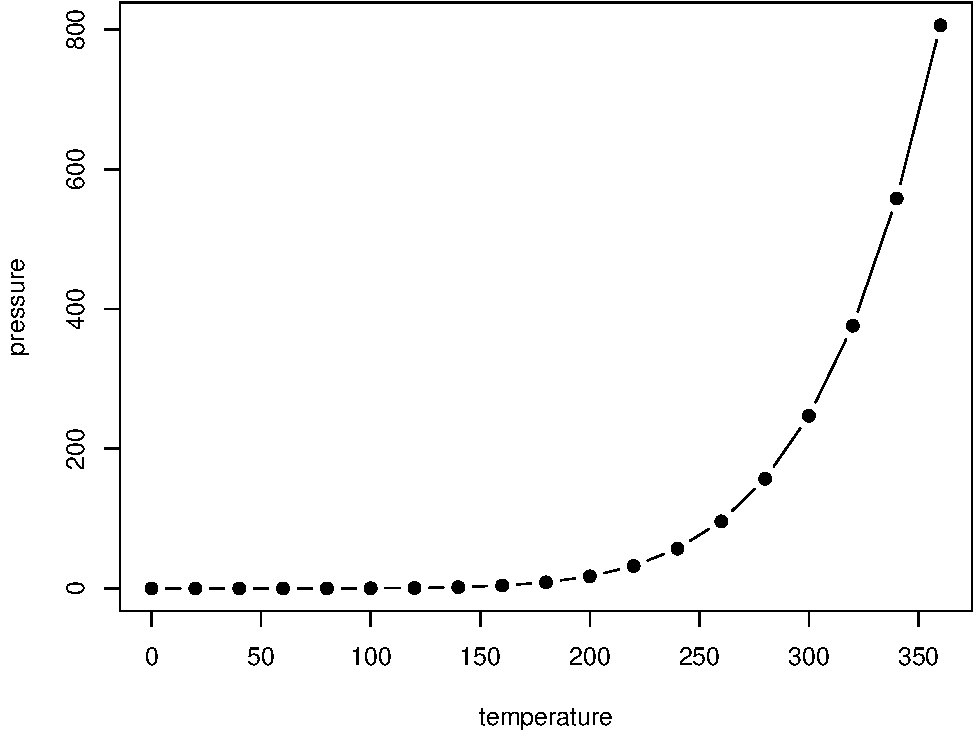
\includegraphics[width=0.8\linewidth]{Lineamientos-Visualizar_files/figure-latex/nice-fig-1} 

}

\caption{Here is a nice figure!}\label{fig:nice-fig}
\end{figure}

Reference a figure by its code chunk label with the \texttt{fig:} prefix, e.g., see Figure \ref{fig:nice-fig}. Similarly, you can reference tables generated from \texttt{knitr::kable()}, e.g., see Table \ref{tab:nice-tab}.

\begin{Shaded}
\begin{Highlighting}[]
\NormalTok{knitr}\OperatorTok{::}\KeywordTok{kable}\NormalTok{(}
  \KeywordTok{head}\NormalTok{(iris, }\DecValTok{20}\NormalTok{), }\DataTypeTok{caption =} \StringTok{'Here is a nice table!'}\NormalTok{,}
  \DataTypeTok{booktabs =} \OtherTok{TRUE}
\NormalTok{)}
\end{Highlighting}
\end{Shaded}

\begin{table}

\caption{\label{tab:nice-tab}Here is a nice table!}
\centering
\begin{tabular}[t]{rrrrl}
\toprule
Sepal.Length & Sepal.Width & Petal.Length & Petal.Width & Species\\
\midrule
5.1 & 3.5 & 1.4 & 0.2 & setosa\\
4.9 & 3.0 & 1.4 & 0.2 & setosa\\
4.7 & 3.2 & 1.3 & 0.2 & setosa\\
4.6 & 3.1 & 1.5 & 0.2 & setosa\\
5.0 & 3.6 & 1.4 & 0.2 & setosa\\
\addlinespace
5.4 & 3.9 & 1.7 & 0.4 & setosa\\
4.6 & 3.4 & 1.4 & 0.3 & setosa\\
5.0 & 3.4 & 1.5 & 0.2 & setosa\\
4.4 & 2.9 & 1.4 & 0.2 & setosa\\
4.9 & 3.1 & 1.5 & 0.1 & setosa\\
\addlinespace
5.4 & 3.7 & 1.5 & 0.2 & setosa\\
4.8 & 3.4 & 1.6 & 0.2 & setosa\\
4.8 & 3.0 & 1.4 & 0.1 & setosa\\
4.3 & 3.0 & 1.1 & 0.1 & setosa\\
5.8 & 4.0 & 1.2 & 0.2 & setosa\\
\addlinespace
5.7 & 4.4 & 1.5 & 0.4 & setosa\\
5.4 & 3.9 & 1.3 & 0.4 & setosa\\
5.1 & 3.5 & 1.4 & 0.3 & setosa\\
5.7 & 3.8 & 1.7 & 0.3 & setosa\\
5.1 & 3.8 & 1.5 & 0.3 & setosa\\
\bottomrule
\end{tabular}
\end{table}

You can write citations, too. For example, we are using the \textbf{bookdown} package \citep{R-bookdown} in this sample book, which was built on top of R Markdown and \textbf{knitr} \citep{xie2015}.

\hypertarget{partes-principales-de-un-gruxe1fico}{%
\chapter{Partes principales de un gráfico}\label{partes-principales-de-un-gruxe1fico}}

A la hora de crear un gráfico es necesario tener presente cada uno de los elementos que lo conforman y determinar cual es la mejor manera de representar cada uno de estos para lograr el impacto deseado en la visualización. El diseño correcto de estos elementos garantizará el éxito de su gráfico, al comunicar de manera acertada la información que pretende presentar. Dentro de la gama de gráficos estadísticos básicos se identifican tres elementos importantes los cuales son ejes, geometría en la cual se incluyen la forma, tamaño y color, tipos de líneas y texto el cual incluye las etiquetas de los ejes, título y leyenda.

\begin{figure}

{\centering 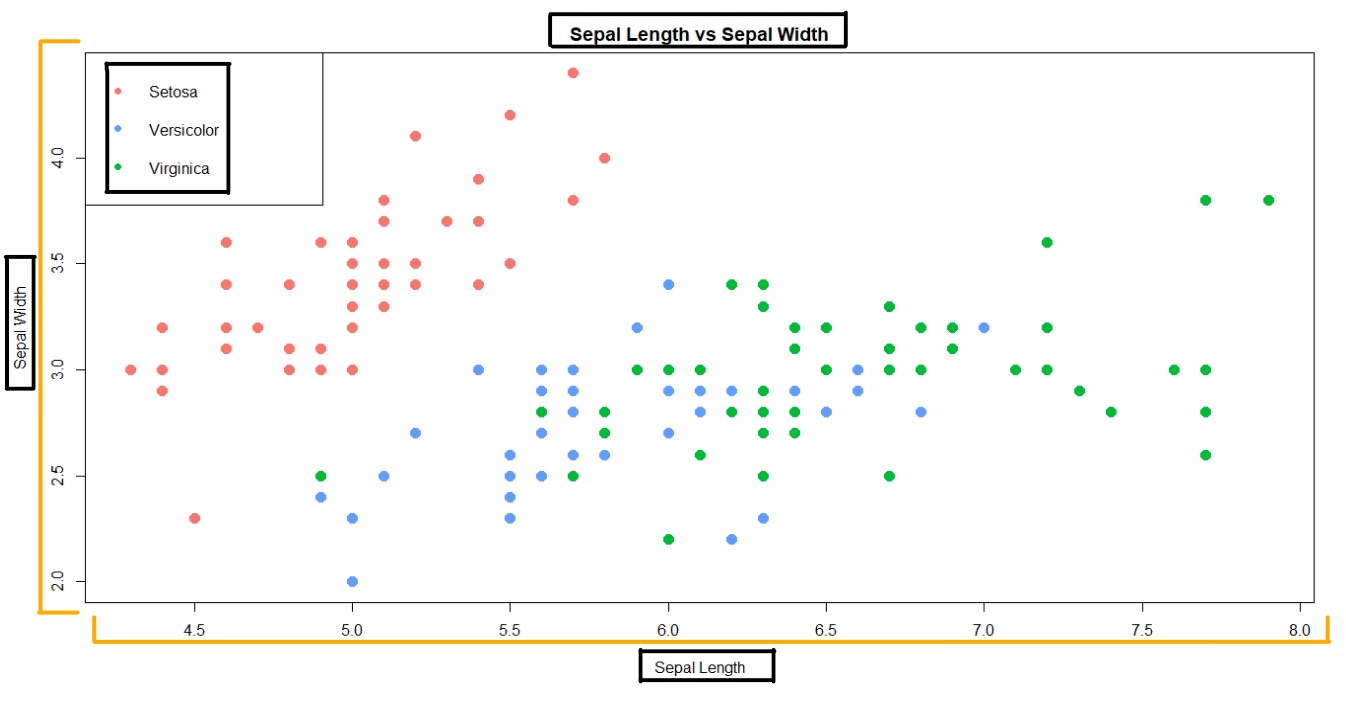
\includegraphics[width=1\linewidth]{Imágenes/partesdelgrafico} 

}

\caption{Principales partes de un gráfico}\label{fig:partesgrafico-fig}
\end{figure}

La figura \ref{fig:partesgrafico-fig} presenta estos elementos importantes. En los recuadros negros se encierra todo lo relacionado con texto, etiquetas de los ejes, título y leyenda; las líneas naranjadas representan los ejes del gráfico de manera horizontal corre el eje X y de manera vertical el eje Y. En la parte central de la visualización se ubican las observaciones a las cuales se les aplica la geometría, dependiendo del tipo de gráfico es posible cambiar el tamaño, forma y color de cado dato.

A continuación, se presentan las características que se consideraron más importantes para tener en cuenta a la hora de dar formato y personalizar cada uno de los elementos mencionados.

\hypertarget{ejes}{%
\section{Ejes}\label{ejes}}

Los ejes son de los elementos de mayor relevancia dentro de cada gráfico ya que determinan la posición donde se ubica cada dato. Cuando se trata de gráficos en dos dimensiones, los más comunes, las posiciones son descritas a través de dos valores que especifican un punto de forma única, y por lo tanto se necesitan escalas de posición, estas escalas son generalmente los ejes X y Y. Por convención general el eje X corre horizontalmente y el eje Y lo hace de manera vertical, aunque esto no siempre debe ser así, hay gráficos en los cuales los ejes son radiales.
El objetivo principal de las visualizaciones que se crean es comparar los datos, es decir, identificar el comportamiento de cada observación en relación con las demás que posee el conjunto de datos. Para realizar estas comparaciones es importante definir la escala de los ejes de manera adecuada, una mala elección de estas escalas lo puede conducir a interpretar la información de manera errada; es recomendable iniciar los ejes en 0, aunque no siempre es necesario si es importante considerar que los datos sean comparables.

Para ilustrar la importancia de la correcta elección del inicio del eje Y consideremos la visualización de cantidades a lo largo de una escala lineal. La figura \ref{fig:usoincorrectoejey-fig} muestra las ventas en cinco estados de EE.UU; una vista rápida a esta visualización indica que las ventas en North Dakota son extremadamente bajas en comparación con los demás estados, sin embargo, este gráfico es engañoso ya que las ventas inician en \(\$900\) USD, por lo tanto, mientras que el punto final de cada barra indica de manera correcta el total de ventas, la altura de la barra representa la medida en que las ventas superan los \(\$900\) dólares; la percepción humana entenderá la altura de cada barra como las ventas por estado lo que conlleva a una interpretación errónea.

\begin{figure}

{\centering 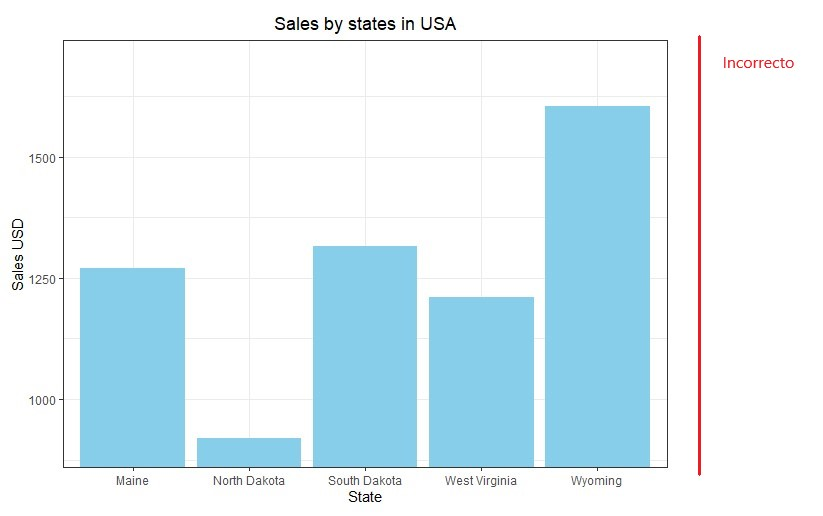
\includegraphics[width=1\linewidth]{Imágenes/iniciarejecero} 

}

\caption{Ventas por estados de EE.UU, visualiazción engañosa}\label{fig:usoincorrectoejey-fig}
\end{figure}

La forma correcta de visualizar estos datos se presenta en la figura \ref{fig:usocorrectoejeyinicio0-fig}, es claro que existen diferencias entre las ventas por estados, pero no son tan distantes como lo muestra la figura \ref{fig:usoincorrectoejey-fig}, las ventas en los cinco estados presentados son comparables. En este caso es particular se debe seguir la regla de iniciar los ejes en cero.

\begin{figure}

{\centering 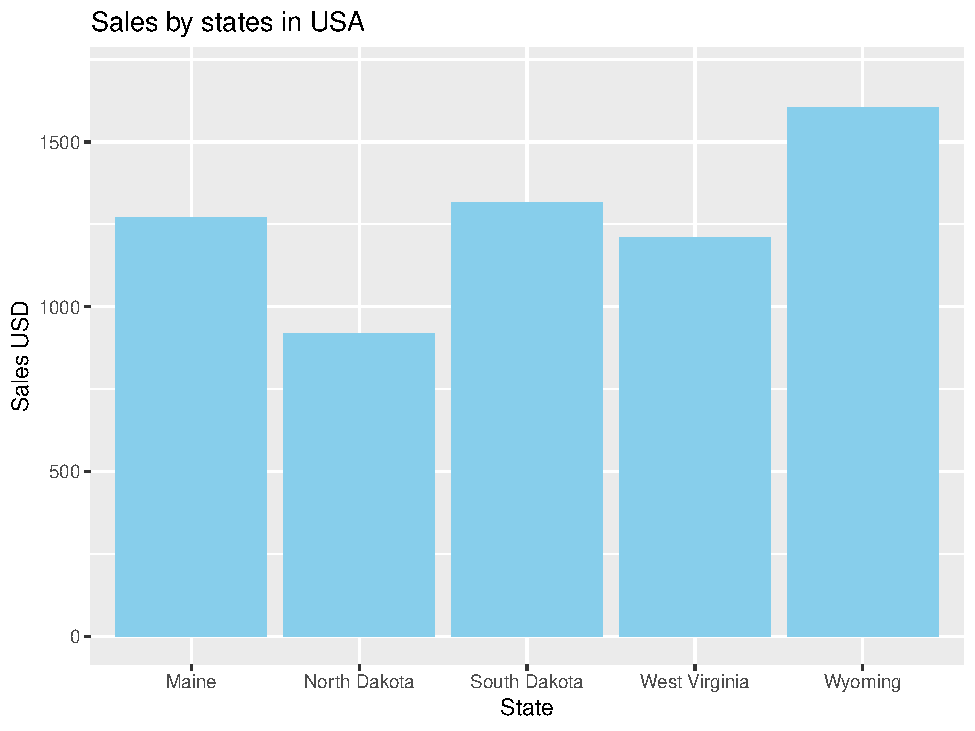
\includegraphics[width=0.8\linewidth]{Lineamientos-Visualizar_files/figure-latex/usocorrectoejeyinicio0-fig-1} 

}

\caption{Ventas por estados de EE.UU, uso correcto de la escala lineal}\label{fig:usocorrectoejeyinicio0-fig}
\end{figure}

Como se mencionó anteriormente no siempre es necesario iniciar los ejes en cero, existen ocasiones en las cuales los datos se encuentran agrupados en un intervalo específico y comenzar los ejes en cero hará que las discrepancias entre los datos no se observen con claridad, la figura \ref{fig:ejeenceroincorrecto-fig} presenta la relación X-Y de datos ficticios, fue etiquetada como incorrecta ya que iniciar el eje Y en cero no permite visualizar con claridad las ubicaciones de los puntos a lo largo del eje vertical.

\begin{figure}

{\centering 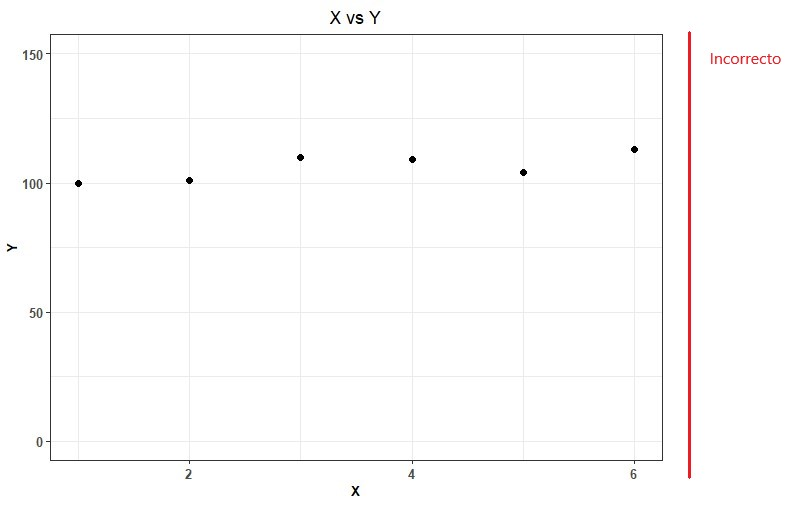
\includegraphics[width=1\linewidth]{Imágenes/incorrectoejeencero} 

}

\caption{Visualización engañosa por iniciar eje en cero}\label{fig:ejeenceroincorrecto-fig}
\end{figure}

En este caso se debe restringir el dominio del eje Y al intervalo 100 a 115 aproximadamente ya que allí es donde se concentran las observaciones, note que la figura \ref{fig:restringirintervalo-fig} es más informativa ya que permite identificar con claridad la ubicación de los puntos dando como resultado una visualización clara y explicativa.

\begin{figure}

{\centering 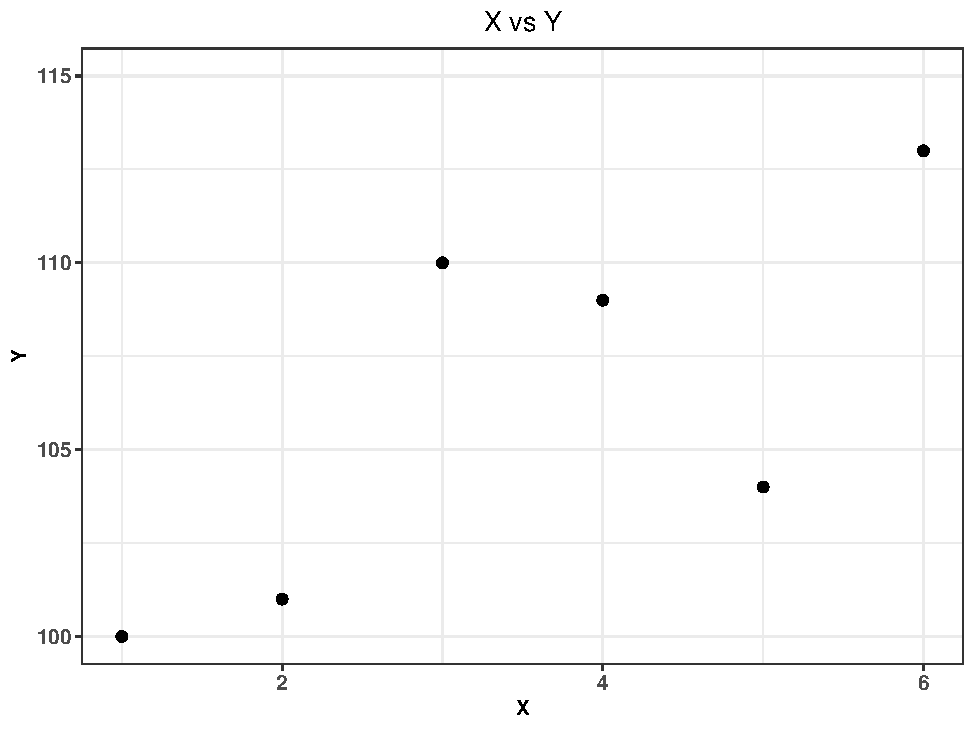
\includegraphics[width=0.8\linewidth]{Lineamientos-Visualizar_files/figure-latex/restringirintervalo-fig-1} 

}

\caption{Restringir dominio del eje Y para una visualización más clara}\label{fig:restringirintervalo-fig}
\end{figure}

\hypertarget{geometruxeda}{%
\section{Geometría}\label{geometruxeda}}

La geometría es una parte primordial y que hará las visualizaciones mucho mas claras y entendibles. Dentro de las geometrías principales podemos considerar la forma, tamaño, tipo de línea y color.

\hypertarget{forma-y-tipo-de-luxednea}{%
\subsection{Forma y tipo de línea}\label{forma-y-tipo-de-luxednea}}

Estas dos son estéticas o atributos que generalmente se usan para representar datos categóricos, dentro de visualizaciones discretas o continuas. Cuando se trata de gráficos de dispersión se opta por usar diferentes formas a partir de una variable categórica con el fin de comparar los comportamientos de cada uno de los valores que toma la variable cualitativa. En el caso de los gráficos de líneas se opta por usar diferentes estilos o tipos de líneas nuevamente con el fin de diferenciar la categoría de los datos, por lo general los estilos usados son líneas continuas y punteadas. Ambos elementos pueden ser usados para distinguir o resaltar, en el caso de ser usados para distinguir se asigna una forma o tipo de línea a cada uno de los niveles de la variable categórica y en el caso de resaltado se usa la misma forma o tipo de línea para todos los datos excepto para aquellos elementos que queremos resaltar.

La figura \ref{fig:formasparadistinguir-fig} ilustra el uso de distintas formas para distinguir las especies de flores registradas en la base de datos Iris. Como ya se menciono se usan tantas formas como niveles tenga la variable categórica, en este caso se usan círculos, triángulos y cuadrados.

\begin{figure}

{\centering 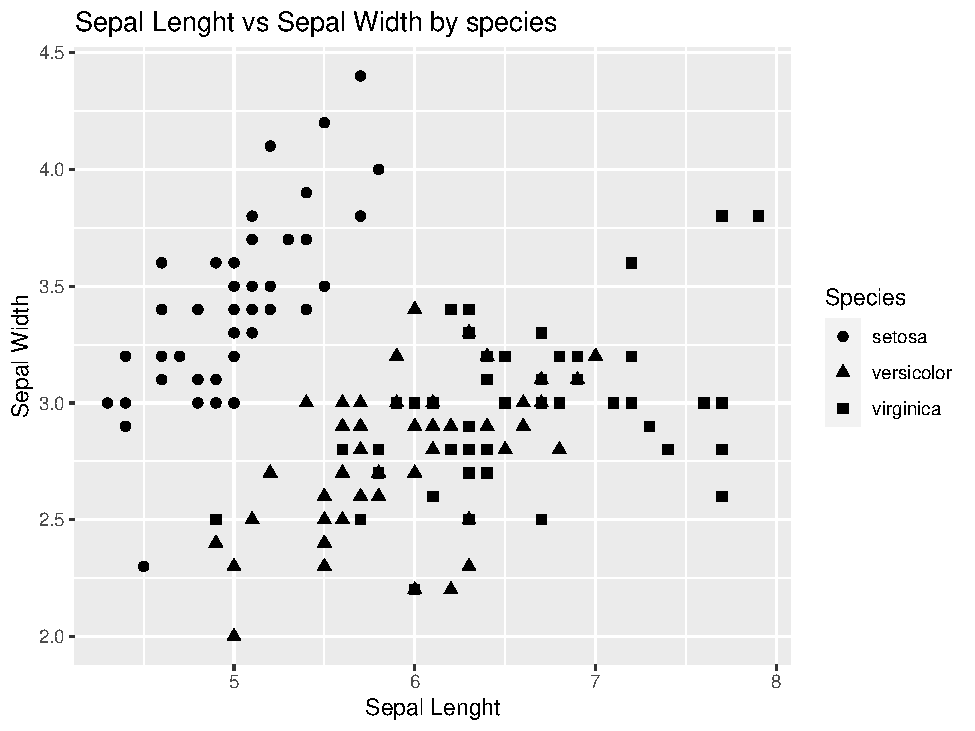
\includegraphics[width=0.8\linewidth]{Lineamientos-Visualizar_files/figure-latex/formasparadistinguir-fig-1} 

}

\caption{Uso de las formas para distinguir grupos de datos}\label{fig:formasparadistinguir-fig}
\end{figure}

Si quisiéramos resaltar una de las especies por ejemplo, Versicolor debemos asignar la misma forma a las especies Setosa y Virginica y una distinta a la especie a resaltar, por ejemplo usar círculos y triángulos, como se presenta en la figura \ref{fig:formaspararesaltar-fig}.

\begin{figure}

{\centering 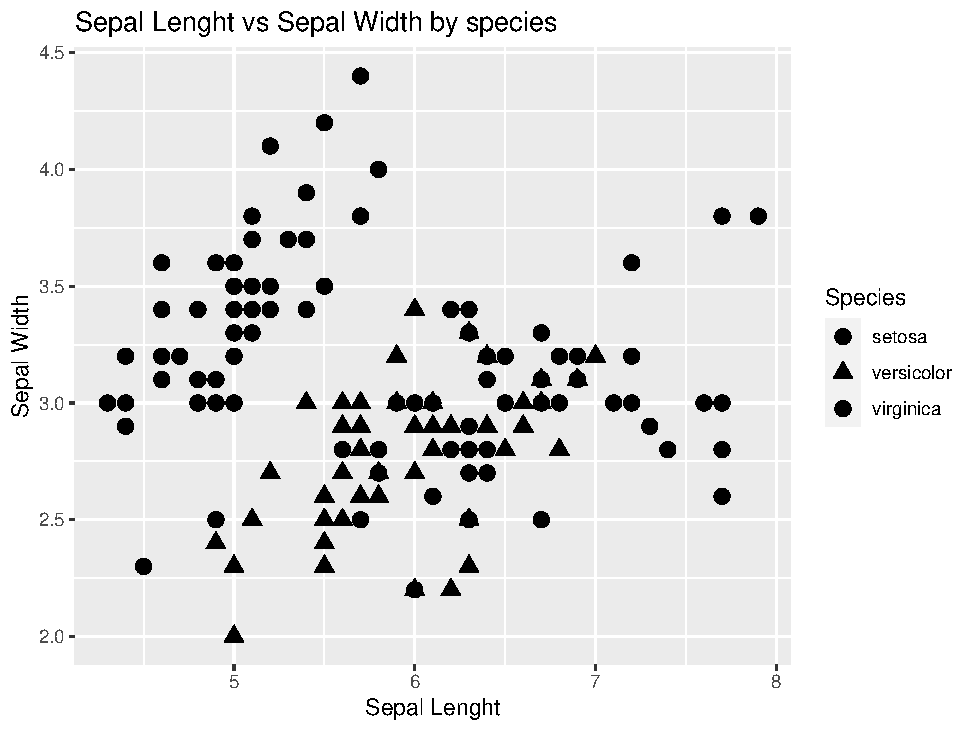
\includegraphics[width=0.8\linewidth]{Lineamientos-Visualizar_files/figure-latex/formaspararesaltar-fig-1} 

}

\caption{Uso de las formas para resaltar un grupo de observaciones}\label{fig:formaspararesaltar-fig}
\end{figure}

Cuando se trata de gráficos de líneas que comúnmente son utilizados para representar series de tiempo también es posible hacer uso del tipo de línea tanto para distinguir como para resaltar, al igual que en los gráficos de dispersión debemos usar tantas formas como categorías tenga la variable discreta si la intención es distinguir. Se usara un conjunto de datos de R llamado babynames que contiene información de la cantidad de bebes nacidos desde el año 1880 hasta 2017 con los respectivos nombres, se realiza un gráfico de líneas con los tres nombres de niñas más populares y se cambia el tipo de línea para distinguir entre nombres como se muestra en la figura \ref{fig:lineasparadistinguir-fig}.

\begin{figure}

{\centering 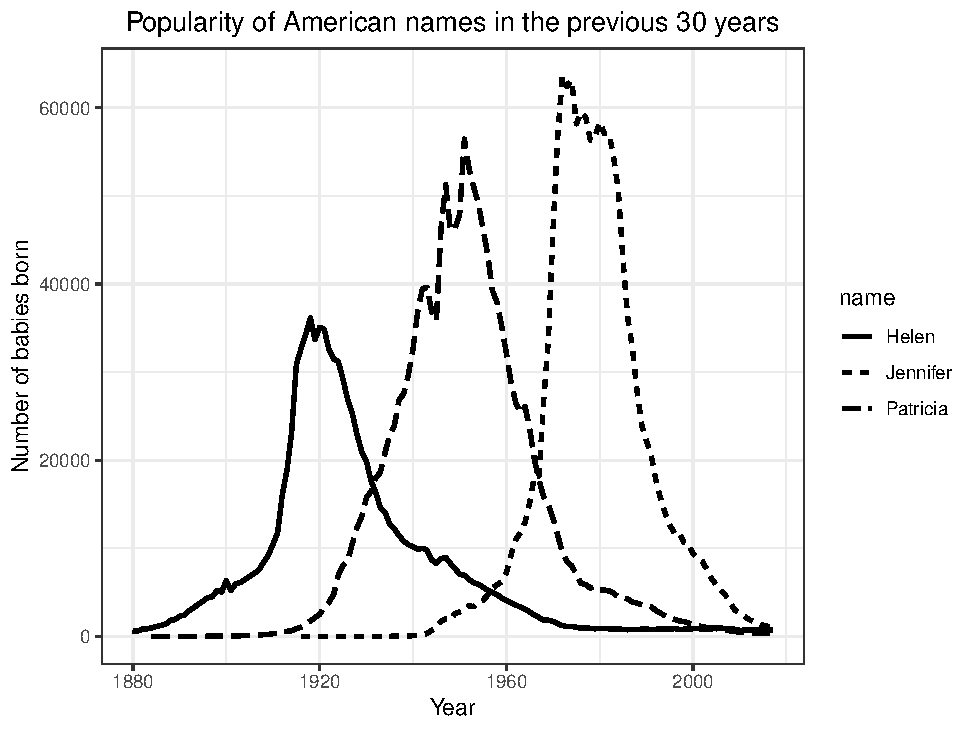
\includegraphics[width=0.8\linewidth]{Lineamientos-Visualizar_files/figure-latex/lineasparadistinguir-fig-1} 

}

\caption{Uso del tipo de líneas para distinguir grupos de observaciones}\label{fig:lineasparadistinguir-fig}
\end{figure}

En el caso de querer resaltar algún nombre en particular debemos usar un tipo de línea diferente para el nombre a resaltar, por ejemplo, en la figura \ref{fig:lineaspararesaltar-fig} se usa una línea punteada para representar la popularidad a través del tiempo del nombre Jennifer y los otros dos se dejaron como líneas continuas.

\begin{figure}

{\centering 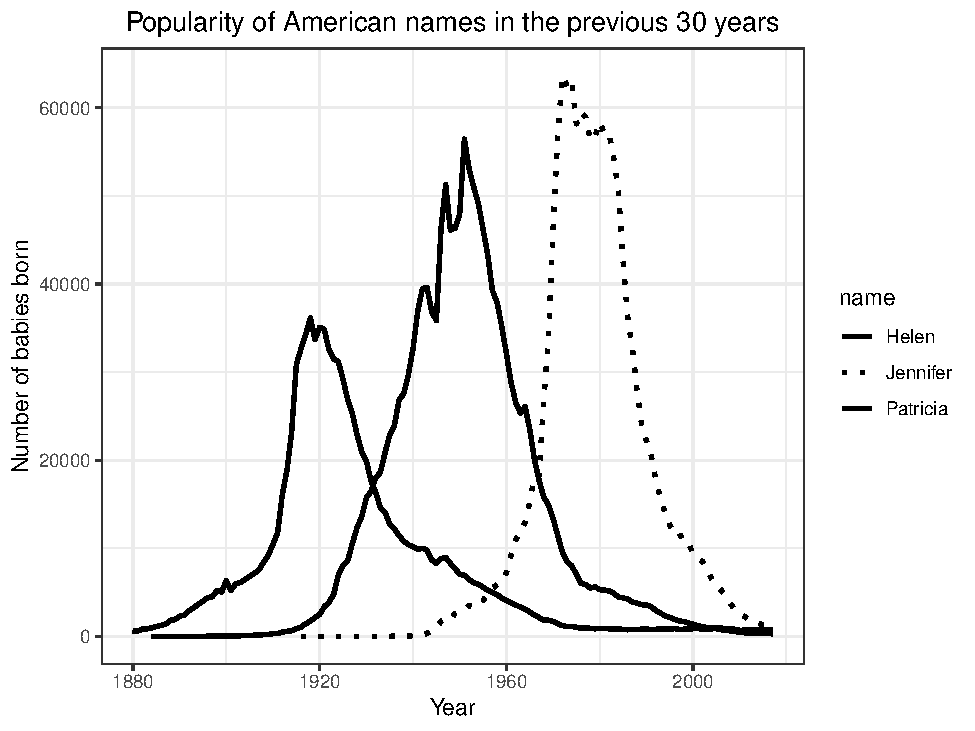
\includegraphics[width=0.8\linewidth]{Lineamientos-Visualizar_files/figure-latex/lineaspararesaltar-fig-1} 

}

\caption{Uso del tipo de líneas para resaltar un grupo de observaciones}\label{fig:lineaspararesaltar-fig}
\end{figure}

Adicional a las formas y tipos de líneas se puede cambiar con el color para generar visualizaciones más atractivas e informativas, ya que al color se le pueden dar distintos usos, esto se muestra en la subsección \ref{colores}.

\hypertarget{tamauxf1o}{%
\subsection{Tamaño}\label{tamauxf1o}}

El tamaño generalmente es una estética usada en gráficos de dispersión, se incluye una nueva variable continua o discreta que determina el tamaño de cada observación representada en el gráfico. Este atributo es de gran utilidad, pero se debe tener mucho cuidado al usarlo, ya que en el caso de datos desproporcionados un solo punto ocupará un tamaño exagerado que será poco comparable con los demás datos.

La figura \ref{fig:usotamanodiscreto-fig} ilustra el uso de una variable discreta para asignar diferentes tamaños a las observaciones.

\begin{figure}

{\centering 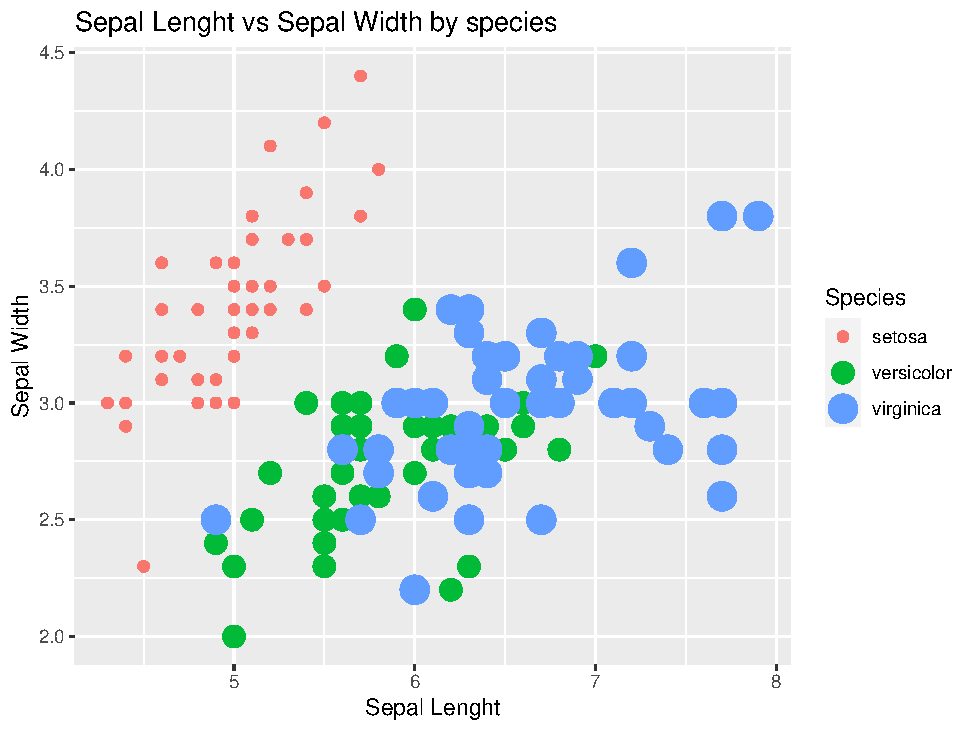
\includegraphics[width=0.8\linewidth]{Lineamientos-Visualizar_files/figure-latex/usotamanodiscreto-fig-1} 

}

\caption{Asignación de tamaños mediante una variable discreta}\label{fig:usotamanodiscreto-fig}
\end{figure}

La figura \ref{fig:usotamanocontinuo-fig} muestra el uso de una variable continua para determinar el tamaño de cada observación, note que a demás de la geometría relacionada al tamaño se debe usar la transparencia para evitar que los países con mayor población oculten o se sobrepongan a aquellos a países de menor población.

\begin{figure}

{\centering 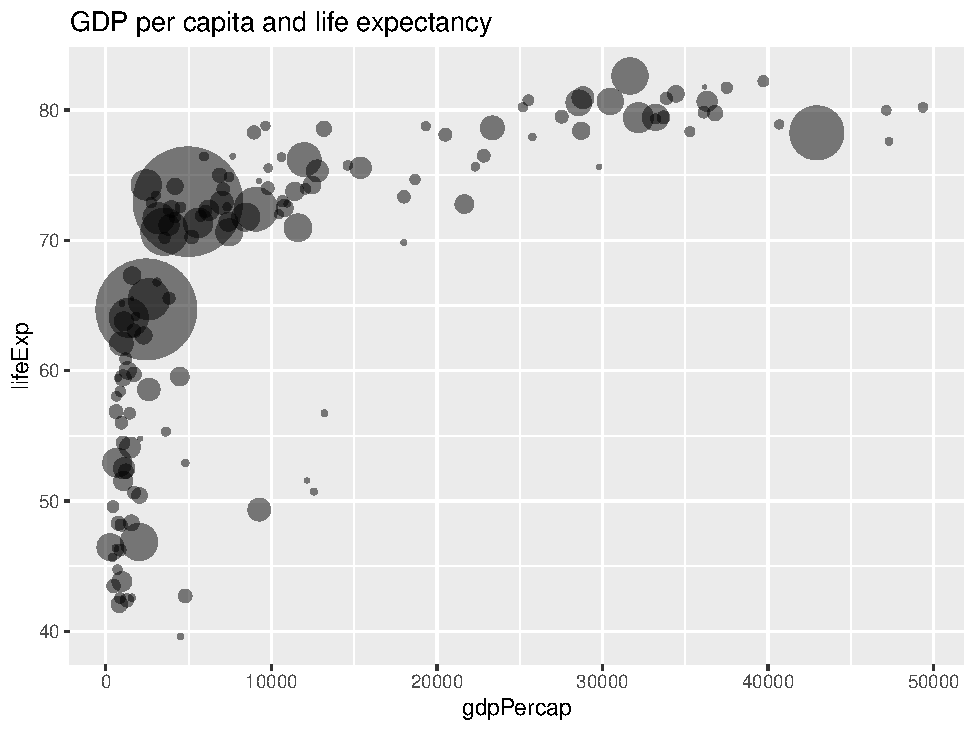
\includegraphics[width=0.8\linewidth]{Lineamientos-Visualizar_files/figure-latex/usotamanocontinuo-fig-1} 

}

\caption{Asignación de tamaños mediante una variable continua}\label{fig:usotamanocontinuo-fig}
\end{figure}

\hypertarget{colores}{%
\subsection{Color}\label{colores}}

El color es una de las estéticas más importantes y que pueden marcar una gran diferencia en la interpretación de sus datos. Existen algunos colores que destacan más que otros por lo que darán un peso innecesario a los datos, es decir, que atraen la atención de los usuarios a esos puntos y que pueden no necesariamente ser los de interés central, también es recomendable no superar los seis colores por gráfico. El color dentro de una visualización puede ser usado principalmente para tres casos: para distinguir grupos de datos entre sí, uso del color para representar valores de datos y finalmente puede ser usado para resaltar.

\hypertarget{distinguir-grupos-de-datos}{%
\subsubsection{Distinguir grupos de datos}\label{distinguir-grupos-de-datos}}

Emplear el color como una herramienta para distinguir es uno de los usos más comunes que se le da al color cuando se trata de gráficos que incluyen variables categóricas y que no tienen un orden específico como diferentes niveles de formación dentro de una universidad o departamentos dentro de un mapa. En este caso, se utiliza una escala de colores cualitativa la cual contiene un conjunto finito de colores específicos que se eligen para versen claramente distintos entre sí y que al mismo tiempo deben ser equivalentes entre sí. Es decir que lo colores seleccionados se deben poder diferenciar de manera clara y precisa, pero uno no debe resaltar más que otro. También es importante que el conjunto de colores seleccionados no presente un orden ya que esto creara un orden en la visualización que por definición de los datos no se tiene. Como recomendación general, las escalas de color cualitativas funcionan mejor cuando hay de tres a cinco categorías diferentes; tener ocho o diez categorías hará que la tarea de hacer coincidir los colores sea tediosa, a demás la leyenda será demasiado extensa y el usuario tendrá que hacer un fuerte trabajo de búsqueda para identificar el color correspondiente a cada categoría; en el caso de muchas categorías se recomienda usar etiquetas directas sobre la observación para así facilitar la comprensión del gráfico aunque con esto también se debe tener cuidado ya que muchas etiquetas hará que la visualización se sature y la información no sea transmitida de la manera correcta.

La figura \ref{fig:usocolordistinguir-fig} muestra el uso correcto de los colores como herramienta para distinguir, se seleccionaron colores que contrastan entre sí pero no compiten por la atención, este gráfico en particular posee ocho categorías distintas pero aún así se logra identificar claramente cada una de las sedes de admisión.

\begin{figure}

{\centering 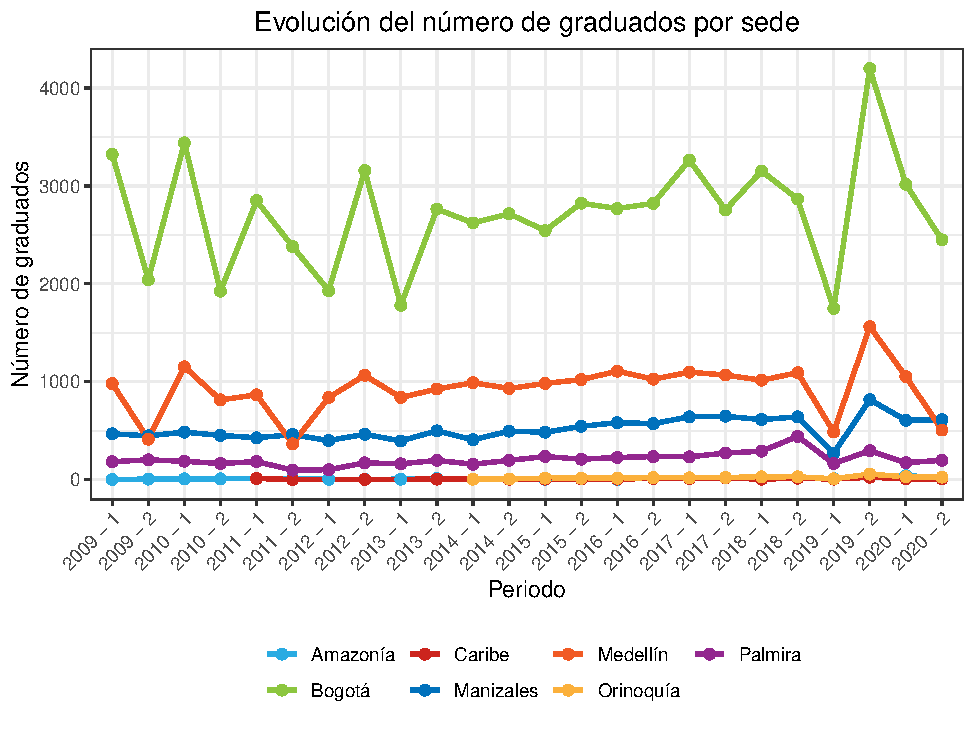
\includegraphics[width=0.9\linewidth]{Lineamientos-Visualizar_files/figure-latex/usocolordistinguir-fig-1} 

}

\caption{Uso del color como herramienta para distinguir grupos de datos}\label{fig:usocolordistinguir-fig}
\end{figure}

\hypertarget{representar-valores}{%
\subsubsection{Representar valores}\label{representar-valores}}

El color también puede ser usado como herramienta para representar variables cuantitativas como ingresos, temperatura, entre otros. En este caso se usa una escala de color secuencial, la cual indica claramente que valores son más grandes o pequeños y que tan distantes se encuentran dos valores específicos entre sí. Estas escalas secuenciales de color pueden basarse en un solo tono por ejemplo de azul oscuro a azul claro, o en múltiples matices por ejemplo de rojo oscuro a amarillo claro.

En la figura \ref{fig:usocolorrepresentar-fig} presenta un uso adecuado de la escala de colores secuencial, se usa una paleta de un solo tono que inicia en azul claro y termina en un azul un poco más fuerte. Esta visualización presenta la cantidad de estudiantes graduados en el periodo 2020-II por departamento de nacimiento y la escala de color fue usada para colorear el conteo por cada uno de estos departamentos.

\begin{figure}

{\centering 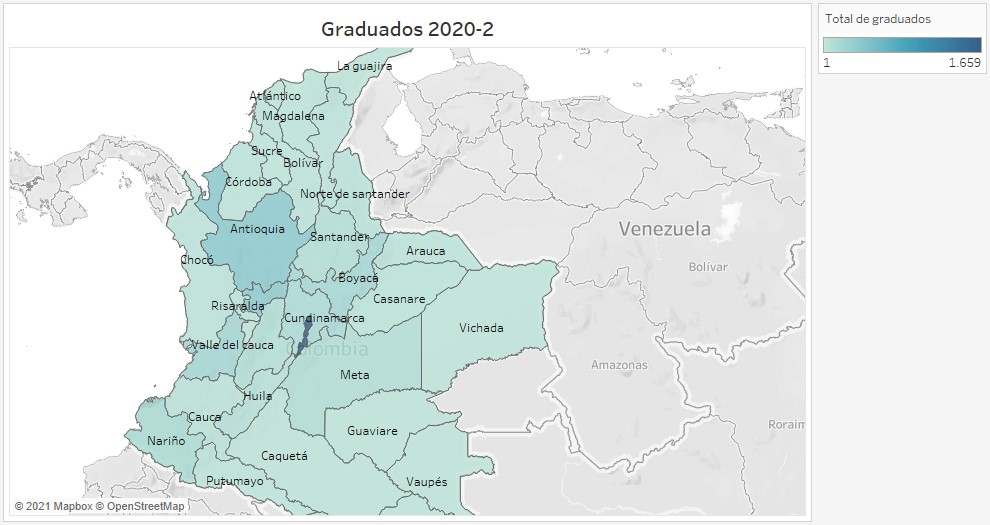
\includegraphics[width=1\linewidth]{Imágenes/escaladecolorsecuencial} 

}

\caption{Uso de la escala de color secuencial para representar valores}\label{fig:usocolorrepresentar-fig}
\end{figure}

Existen algunas ocasiones en las cuales es necesario visualizar la desviación de los valores de los datos en una de dos direcciones en relación con un punto medio neutral. Un ejemplo sencillo y muy básico de estos casos es cuando se tienen números positivos y negativos, que se representan por dos colores, puede ser verde para los números positivos y rojo para los negativos, a partir de la intensidad de estos colores se indica la lejanía con el cero. La escala de color usada en estos casos se denomina divergente y puede pensarse como dos escalas de colores secuenciales que se unen en un punto medio; estas escalas deben ser equilibradas, de modo que la progresión de los colores claros en el centro a los colores oscuros del exterior debe ser la aproximadamente igual para ambas direcciones.

\begin{figure}

{\centering 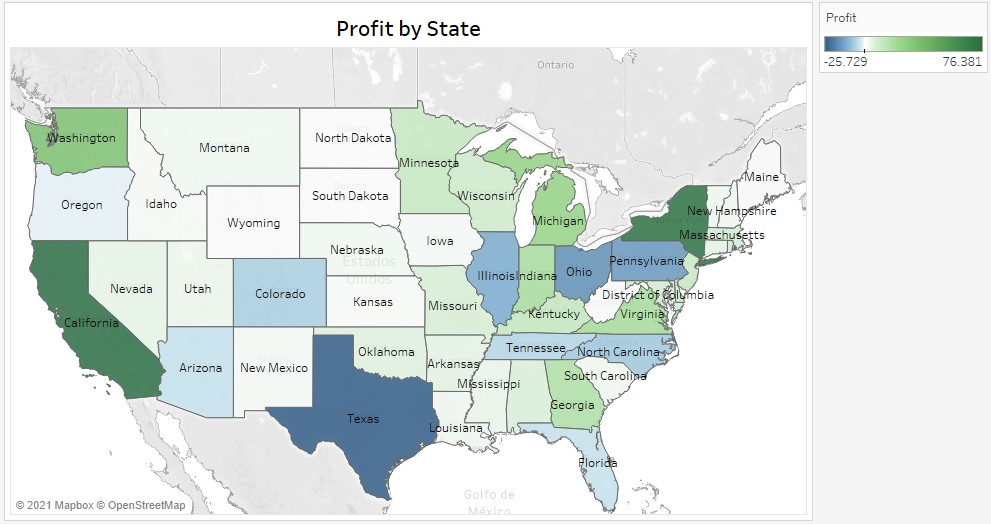
\includegraphics[width=1\linewidth]{Imágenes/escaladivergente} 

}

\caption{Escala divergente para representar valores}\label{fig:escaladivergente-fig}
\end{figure}

La figura \ref{fig:escaladivergente-fig} presenta una de los tantos usos que se le puede dar a las escalas de colores divergentes, se presenta los beneficios por estados. Es importante notar que la escala de colores no se encuentra equilibrada y esto se debe a la desproporción de los datos, a pesar de esto la visualización sigue siendo informativa y se logra distinción entre los colores.

\hypertarget{resaltar-observaciones}{%
\subsubsection{Resaltar observaciones}\label{resaltar-observaciones}}

Emplear el color para resaltar observaciones es de gran utilidad cuando el conjunto de datos contiene información clave sobre la historia que se quiere contar a través del gráfico y enfatizar en estos elementos conlleva a una mejor comprensión de la información que se desea comunicar. Para lograr este énfasis podemos colorear estos elementos de la figura con colores o tonalidades que se destaquen vívidamente contra el resto de la figura; generalmente se usan escalas de color de acento, las cuales contienen tanto un conjunto de colores tenues como un conjunto coincidente de colores más fuertes.

Cuando se trabaja con una escala de color de acento, es fundamental que los colores básicos no compitan por la atención. Estos colores de base deben ser monótonos pero que apoye bien el color de acento, es muy común cometer el error de usar colores de línea de base que son demasiado coloridos, de modo que terminan compitiendo por la atención del lector. Una alternativa fácil es usar un color neutro en todos los elementos de la figura, excepto para la categoría de puntos que se quiere resaltar.

La figura \ref{fig:resaltardatos-fig} muestra el total de estudiantes admitidos por departamento de nacimiento, se hace uso de una escala de color de acento para resaltar los departamentos pertenecientes a la región andina. Observe que se usa un color neutro para los departamentos que no son de interés y un color azul llamativo para atraer la atención del usuario a la región andina. Esta figura presenta uno de los tantos usos que se le puede dar a las escalas de colores de acento para resaltar datos, es posible aplicarla a gráficos de líneas, diagramas de dispersión, entre otros.

\begin{figure}

{\centering 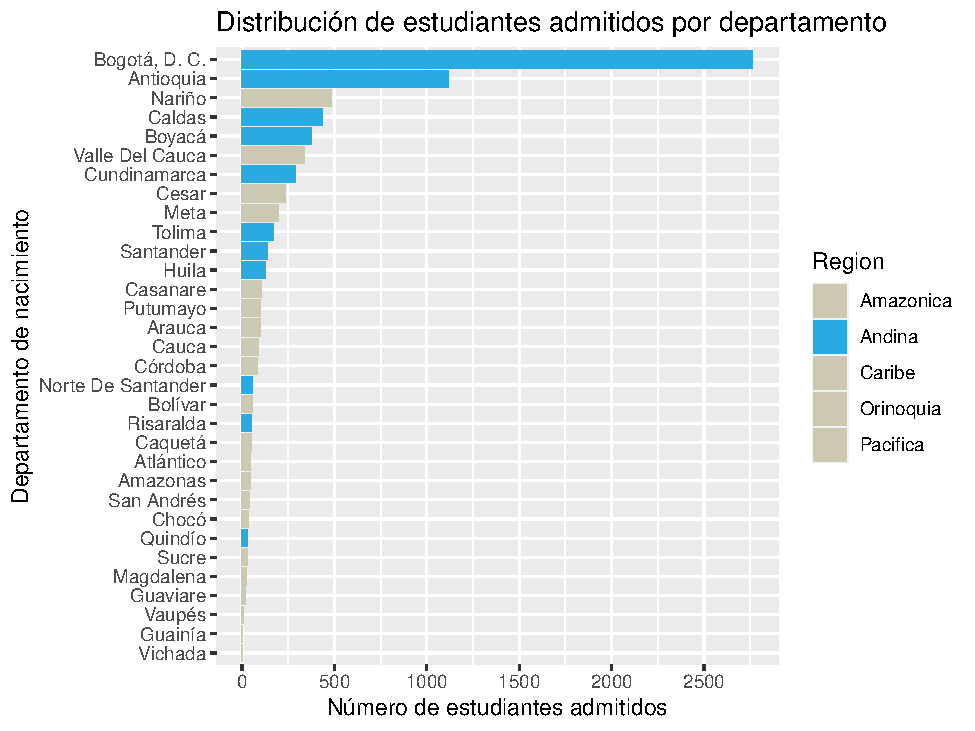
\includegraphics[width=0.8\linewidth]{Lineamientos-Visualizar_files/figure-latex/resaltardatos-fig-1} 

}

\caption{Escala de color de acento para resaltar observaciones}\label{fig:resaltardatos-fig}
\end{figure}

\hypertarget{texto}{%
\section{Texto}\label{texto}}

Al momento de realizar una visualización el texto es uno de los elementos a los cuales se les presta poca atención pero que podrían hacer el gráfico aún mas informativo, se debe manejar una misma fuente pero proporcionar un balance entre los tamaños con el fin de destacar los elementos importantes, por ejemplo, el título de la visualización debe atraer más la atención del usuario que las etiquetas del eje por esta razón no es correcto utilizar un tamaño mayor para las etiquetas del eje que para el título. El éxito de la estética de este elemento se basa en establecer correctamente la jerarquía que existe entre los textos que involucra el gráfico.

El objetivo principal de una visualización es informar y transmitir información de manera clara y concisa, por esta razón se deben colocar los datos en contexto proporcionando títulos, subtítulos y otras anotaciones que los acompañen. A continuación, analizaremos algunas recomendaciones utiles que nos ayudarán a contextualizar los datos de manera correcta.

Uno de los elementos principales dentro de un gráfico es su título, este debe ser claro e informativo ya que su función es transmitir con precisión al lector de qué se trata la figura, también existen ocasiones en las que es necesario usar subtítulos para contextualizar por completo al usuario acerca de la información que se presenta. Otro elemento importante y que logra que las visualizaciones se expliquen por sí mismas son los títulos de los ejes, estos deben indicar de manera clara lo que representan y la unidad en que se miden, observe la figura \ref{fig:usocorrectoejeyinicio0-fig} en la cual el eje Y esta titulado de manera correcta ya que indica que representa las ventas y esta medido en dólares; los títulos de las leyendas también deben ser claros e indicar lo que representan como se muestra en la figura \ref{fig:resaltardatos-fig}, donde el título de la leyenda hace referencia a la región geográfica del país, en algunas ocasiones es posible omitir el título de los ejes o de las leyendas, es decir, cuando las etiquetas son completamnete explícitas.

La figura \ref{fig:usoincorrectotextos-fig} ilustra lo que no se debe hacer en una visualización ya que se le da enfoque princical a las etiquetas del eje y leyenda y no al título de la figura, el cual informa acerca de la visualización.

\begin{figure}

{\centering 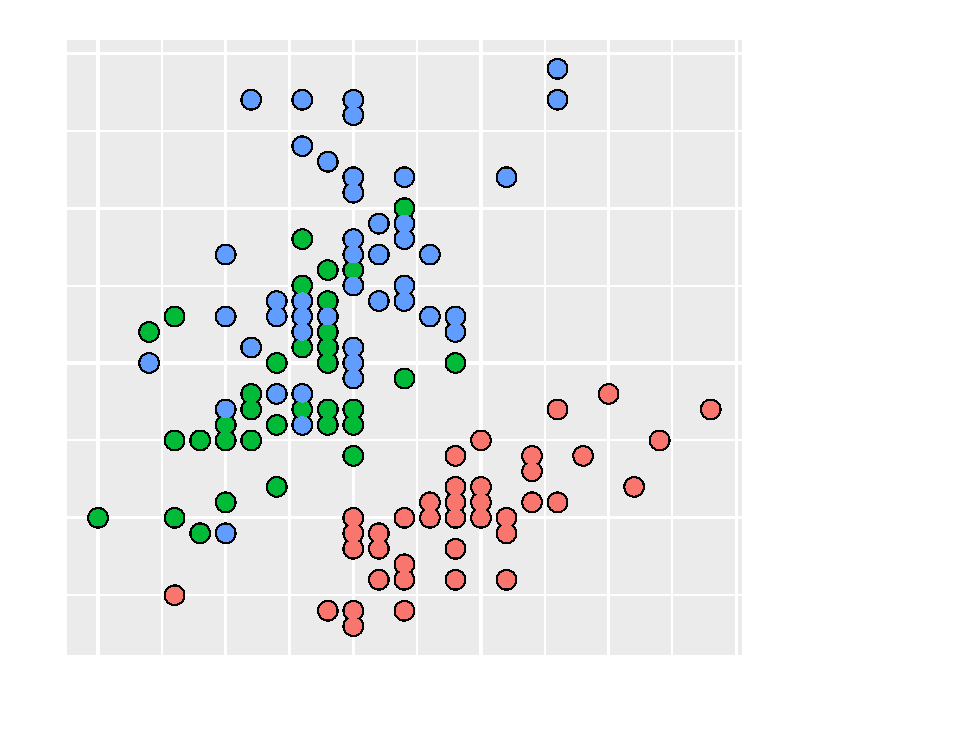
\includegraphics[width=0.8\linewidth]{Lineamientos-Visualizar_files/figure-latex/usoincorrectotextos-fig-1} 

}

\caption{Uso incorrecto del texto}\label{fig:usoincorrectotextos-fig}
\end{figure}

La figura \ref{fig:manejotextos-fig} presenta la clara jerarquía existente entre los textos del gráfico, observe que se trabaja con la misma fuente pero se juega con mayúsculas y minúsculas para dar la importancia que cada elemento requiere, esta visualización es un ejemplo en el cual se puede omitir el título de la leyenda, ya que las etiquetas son tan claras que usar un título conlleva a un gráfico saturado.

\begin{figure}

{\centering 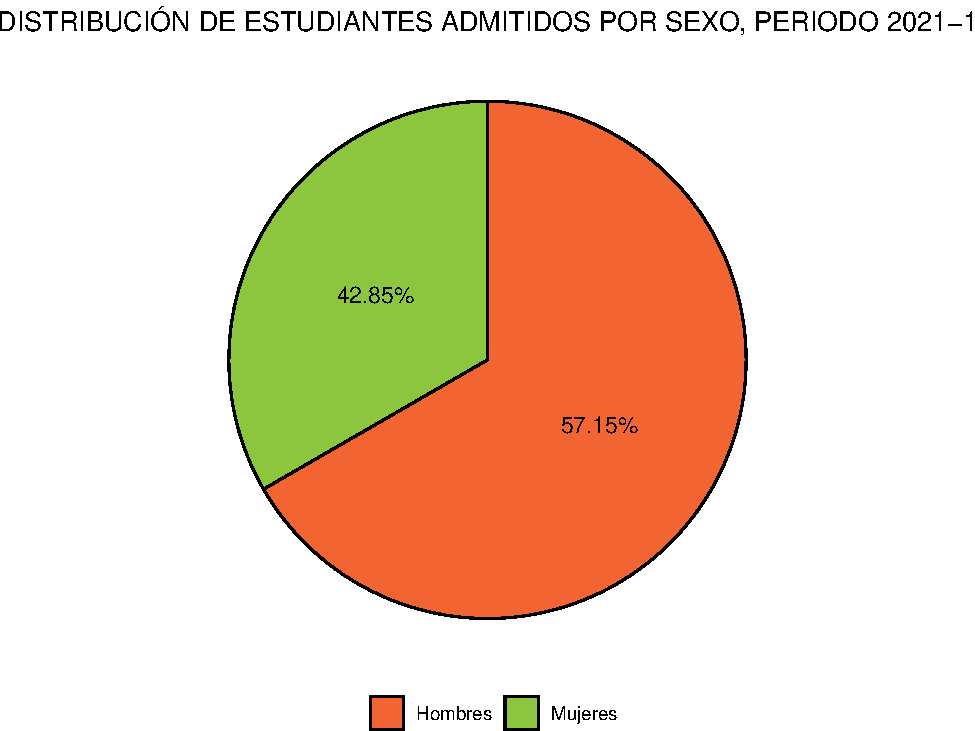
\includegraphics[width=0.8\linewidth]{Lineamientos-Visualizar_files/figure-latex/manejotextos-fig-1} 

}

\caption{Uso correcto del texto para contextualizar}\label{fig:manejotextos-fig}
\end{figure}

\hypertarget{cuxf3mo-visualizar-los-datos}{%
\chapter{¿Cómo visualizar los datos?}\label{cuxf3mo-visualizar-los-datos}}

En la actualidad hay muchos gráficos disponibles para visualizar nuestros datos, pero no todos los gráficos pueden ser usados para lo que se quiere representar, por esta razón es importante conocer cuáles son los gráficos apropiados para los datos que se quieren mostrar. Dentro de los datos más comunes a visualizar se tienen las cantidades, proporciones, distribuciones, series de tiempo, datos geoespaciales, relaciones X-Y e indicadores hacia una meta en particular.

En este capítulo se presenta la forma correcta de representar estos datos con los gráficos que se tienen disponibles, teniendo el contraste entre lo correcto e incorrecto con el fin de informar al usuario acerca de lo que se debe o no hacer para crear las visualizaciones.

\hypertarget{visualizaciuxf3n-de-cantidades}{%
\section{Visualización de cantidades}\label{visualizaciuxf3n-de-cantidades}}

En muchas ocasiones estamos interesados en visualizar la magnitud de algún conjunto de números, por ejemplo, visualizar el volumen de ventas por estados, total de estudiantes admitidos por modalidad de formación, estudiantes graduados por grupos de edad o departamento, entre muchos otros ejemplos. Observe que en todos estos casos se tiene un conjunto de categorías y un valor cuantitativo para cada categoría. La visualización recomendada y más usada en este escenario es el gráfico de barras en el cual se incluyen distintas variaciones tales como las barras simples, agrupadas y apiladas tanto verticales como horizontales. Las alternativas al diagrama de barras son los diagramas de puntos y mapas de calor.

\hypertarget{gruxe1fico-de-barras}{%
\subsection{Gráfico de barras}\label{gruxe1fico-de-barras}}

Suponga que queremos visualizar la cantidad de estudiantes de estudiantes admitidos por nivel de formación para el periodo 2021-1, este tipo de datos se visualiza comúnmente con barras verticales, para cada nivel de formación se dibuja una barra que inicia en cero y se extiende hasta la cantidad de estudiantes admitidos. La figura \ref{fig:barrasadmitidosnivel-fig} muestra el uso del gráfico de barras para visualizar estas cantidades.

\begin{figure}

{\centering 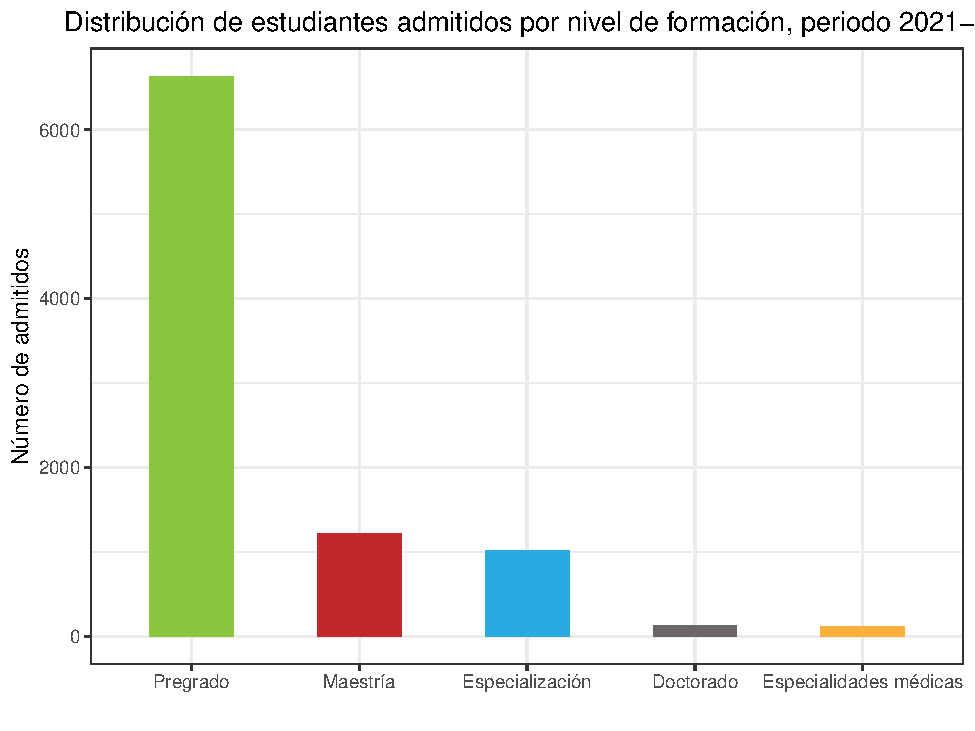
\includegraphics[width=0.8\linewidth]{Lineamientos-Visualizar_files/figure-latex/barrasadmitidosnivel-fig-1} 

}

\caption{Uso del gráfico de barras para representar cantidades}\label{fig:barrasadmitidosnivel-fig}
\end{figure}

Uno de los problemas más comunes con los gráficos de barras verticales es que las etiquetas que identifican cada barra ocupan mucho espacio horizontal. Por esta razón en la figura \ref{fig:barrasadmitidosnivel-fig} fue necesario aumentar la separación entre las barras para poder ubicar las etiquetas en la parte inferior de cada barra y que estas no se traslaparan. Una solución a este problema es girar las etiquetas de cada barra como se muestra en la figura \ref{fig:barrasadmitidosnivelgirar-fig}, pero esto no es estéticamente correcto, ya que es incómodo para el usuario.

\begin{figure}

{\centering 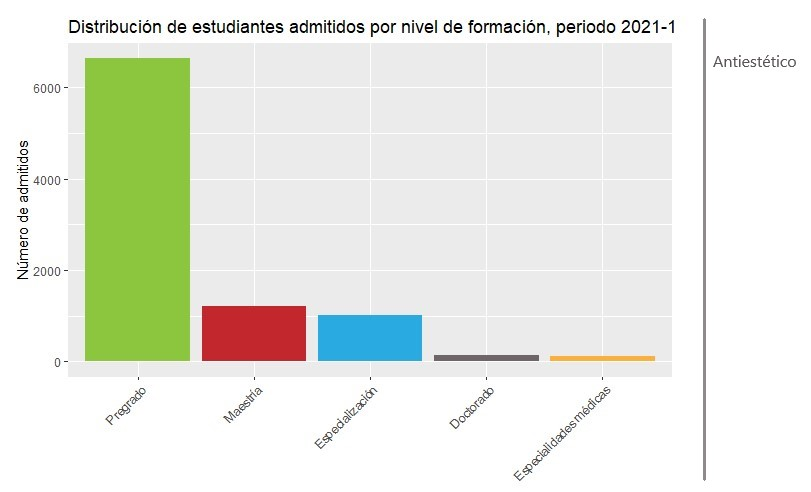
\includegraphics[width=1\linewidth]{Imágenes/etiquetasgiradas} 

}

\caption{Uso del gráfico de barras para representar cantidades, girando etiquetas}\label{fig:barrasadmitidosnivelgirar-fig}
\end{figure}

La mejor solución para etiquetas largas es cambiar a un gráfico de barras horizontales, de esta manera no será necesario aumentar el espaciado entre barras ni girar las etiquetas y se obtiene una visualización compacta en la cual todos los elementos visuales están ubicados de manera horizontal y hace que el gráfico sea más fácil de leer.

\begin{figure}

{\centering 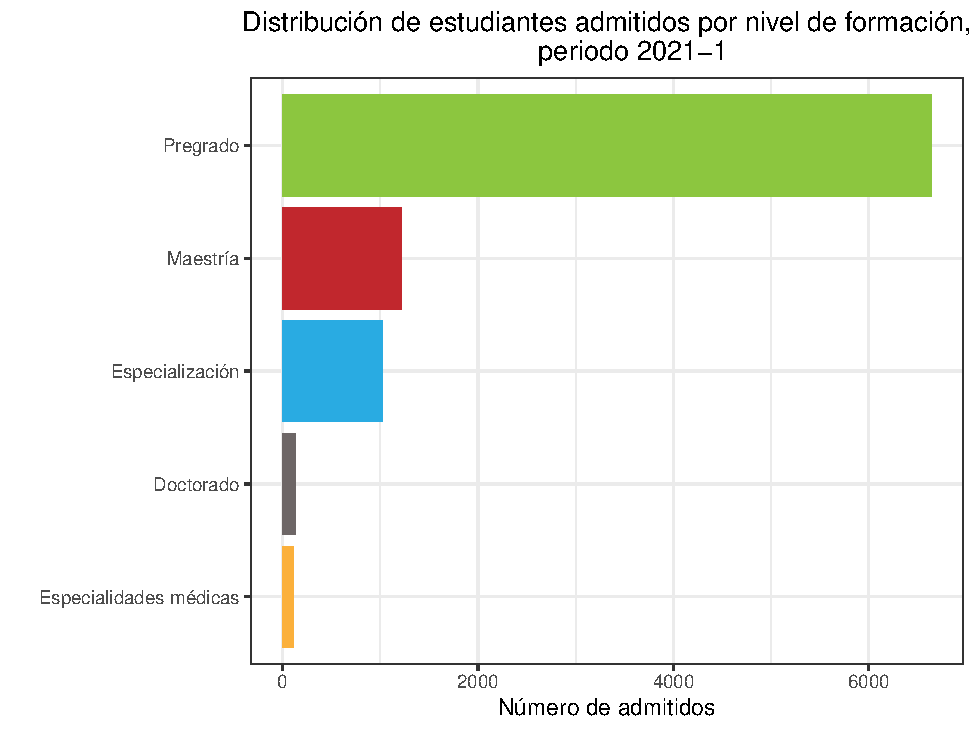
\includegraphics[width=0.8\linewidth]{Lineamientos-Visualizar_files/figure-latex/barrasadmitidosnivelhorizontal-fig-1} 

}

\caption{Uso del gráfico de barras horizontales para representar cantidades}\label{fig:barrasadmitidosnivelhorizontal-fig}
\end{figure}

Sin importar la posición de las barras es decir si son horizontales o verticales se debe prestar mucha atención al orden en el cual se ubica cada barra, en muchas ocasiones las barras están dispuestas de forma arbitraria o por algún criterio que no es significativo en el contexto de la figura, algunos programas simplemente ubican las etiquetas por orden alfabético o algún otro criterio.

Sin embargo, las etiquetas solo pueden ser reordenadas cuando las categorías que representan no tienen un orden natural establecido. Siempre que exista un orden natural en los datos es necesario mantener este orden para representar los datos de la manera correcta. Suponga que se desea visualizar la cantidad de estudiantes graduados en el periodo 2020-2 por grupos de edad. En este caso las barras deben ordenarse de manera creciente según el grupo de edad como se ilustra en la figura \ref{fig:graduadosporgrupoedad-fig}. En este caso no tiene sentido ordenar por la altura de la barra, es decir de forma ascendente o descendente ya que las etiquetas perderán el orden natural que poseen.

\begin{figure}

{\centering 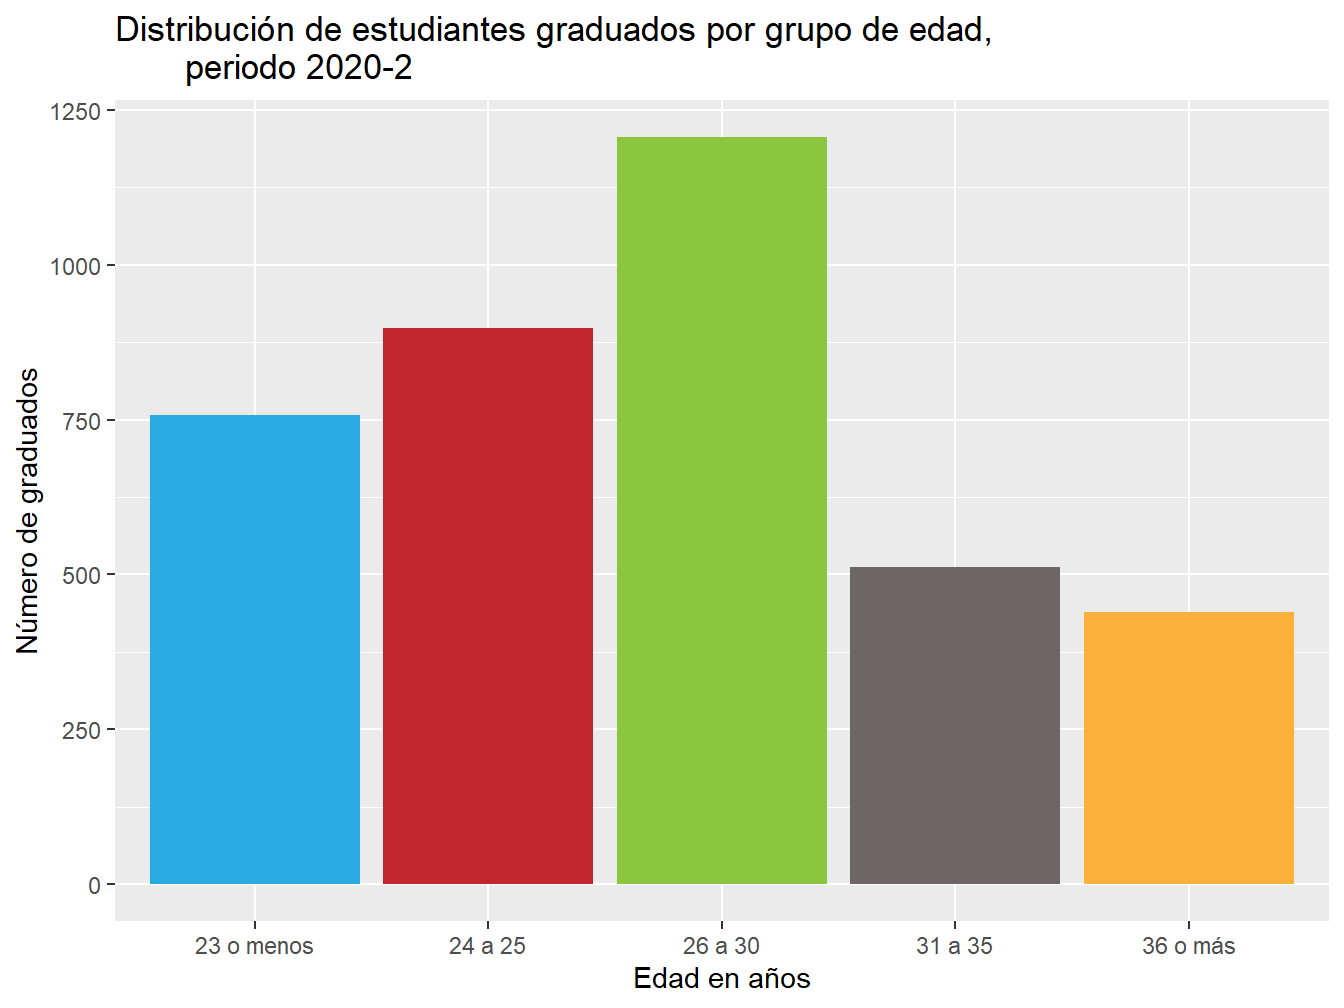
\includegraphics[width=0.8\linewidth]{Lineamientos-Visualizar_files/figure-latex/graduadosporgrupoedad-fig-1} 

}

\caption{Etiquetas con un orden natural}\label{fig:graduadosporgrupoedad-fig}
\end{figure}

\begin{figure}

{\centering 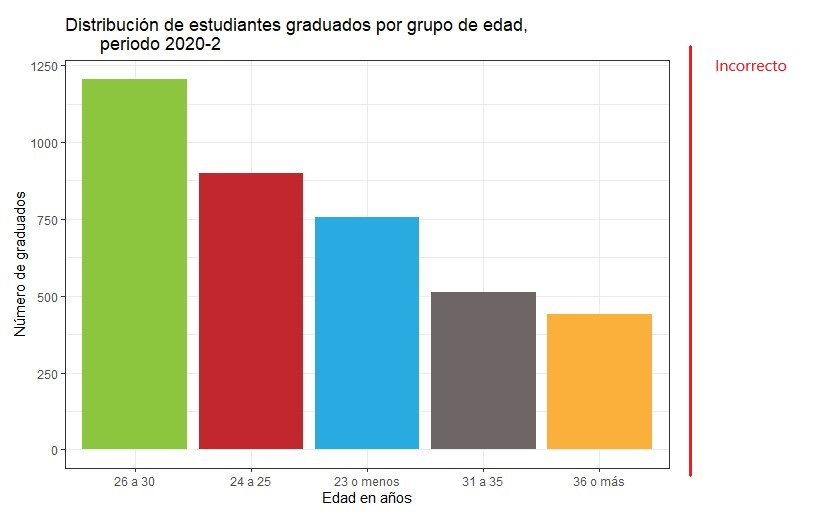
\includegraphics[width=1\linewidth]{Imágenes/ordenarbarrasincorrectas} 

}

\caption{Reordenar etiquetas cuando se tiene un orden natural}\label{fig:partesgrafico2-fig}
\end{figure}

\hypertarget{barras-agrupadas-y-apiladas}{%
\subsection{Barras agrupadas y apiladas}\label{barras-agrupadas-y-apiladas}}

Las figuras mostradas en la subsección anterior representan variables cualitativas en relación con una variable categórica. Sin embargo, a menudo es de interés visualizar como estos valores varían según dos variables categóricas; en un diagrama de barras apiladas, se dibuja un grupo de barras en cada posición del eje X, determinado por una variable categórica, y luego se dibujan barras dentro de cada grupo con la otra variable categórica de interés, por ejemplo, es posible representar el número de funcionarios adminsitrativos por años de servicio prestado y sexo para el periodo 2020-2 tal y como se ilustra en la figura \ref{fig:barrasagrupadasservicioedad-fig}.

\begin{figure}

{\centering 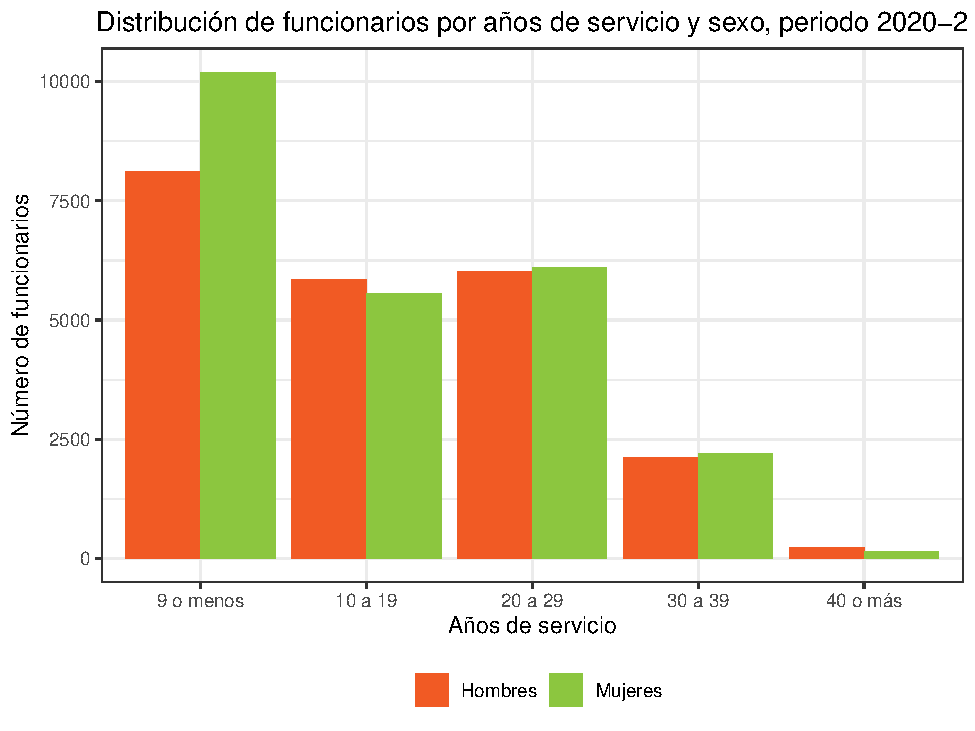
\includegraphics[width=0.8\linewidth]{Lineamientos-Visualizar_files/figure-latex/barrasagrupadasservicioedad-fig-1} 

}

\caption{Uso de barras agrupadas para representar valores usando dos categorías}\label{fig:barrasagrupadasservicioedad-fig}
\end{figure}

Con los gráficos de barras agrupadas se debe tener cuidado ya que las variables categóricas elegidas pueden tener muchos niveles y harán que le gráfico se sature y el usuario no comprenda la información de manera correcta, la figura \ref{fig:barrasagrupadasserviciosede-fig} muestra la distribución del número de funcionarios por años de servicio y sede para el periodo 2020-2, aunque la figura es correcta resulta difícil de interpretar por la cantidad de sedes existentes dentro de la Universidad Nacional de Colombia, observe que para cada grupo de años de servicio se crean diez barras

\begin{figure}

{\centering 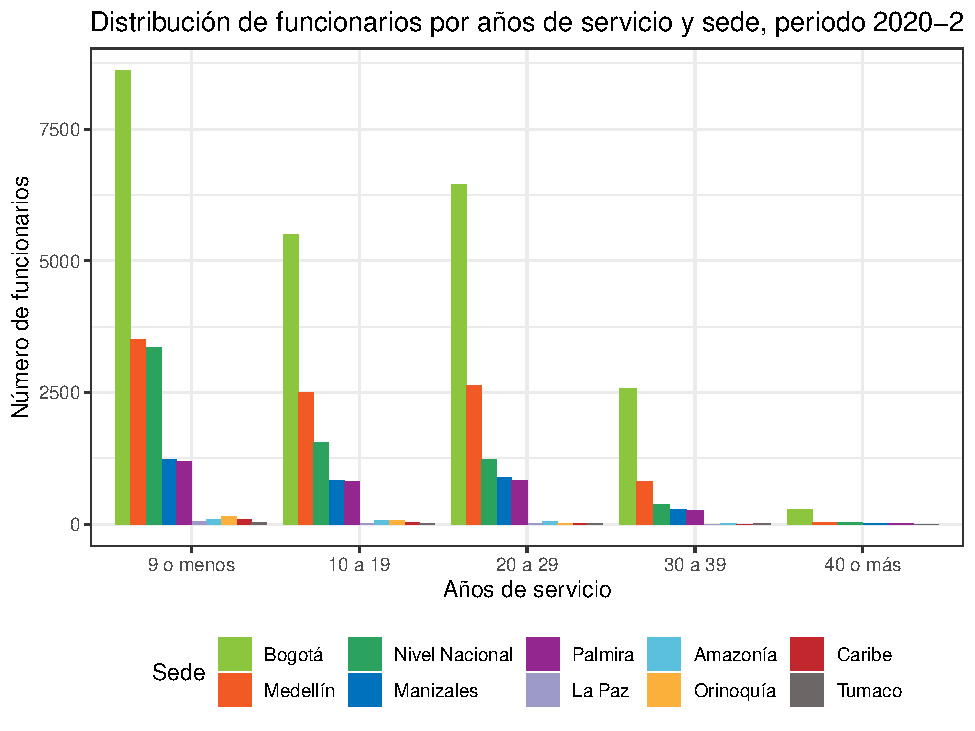
\includegraphics[width=0.8\linewidth]{Lineamientos-Visualizar_files/figure-latex/barrasagrupadasserviciosede-fig-1} 

}

\caption{Cantidad de funcionarios por años de servicio y sede}\label{fig:barrasagrupadasserviciosede-fig}
\end{figure}

Una alternativa a esta figura es visualizar como categoría principal la sede a la que pertenece cada funcionario y que los grupos de barras para cada sede se creen a partir de los años de servicio prestados, usando una escala de color secuencial para representar cada uno de los años de servicio prestado por los funcionarios administrativos, con esto solo se tendrán 5 barras por cada sede y el gráfico será más sencillo y comprensible, como se muestra en la figura \ref{fig:barrasagrupadassedeservicio-fig}.

\begin{figure}

{\centering 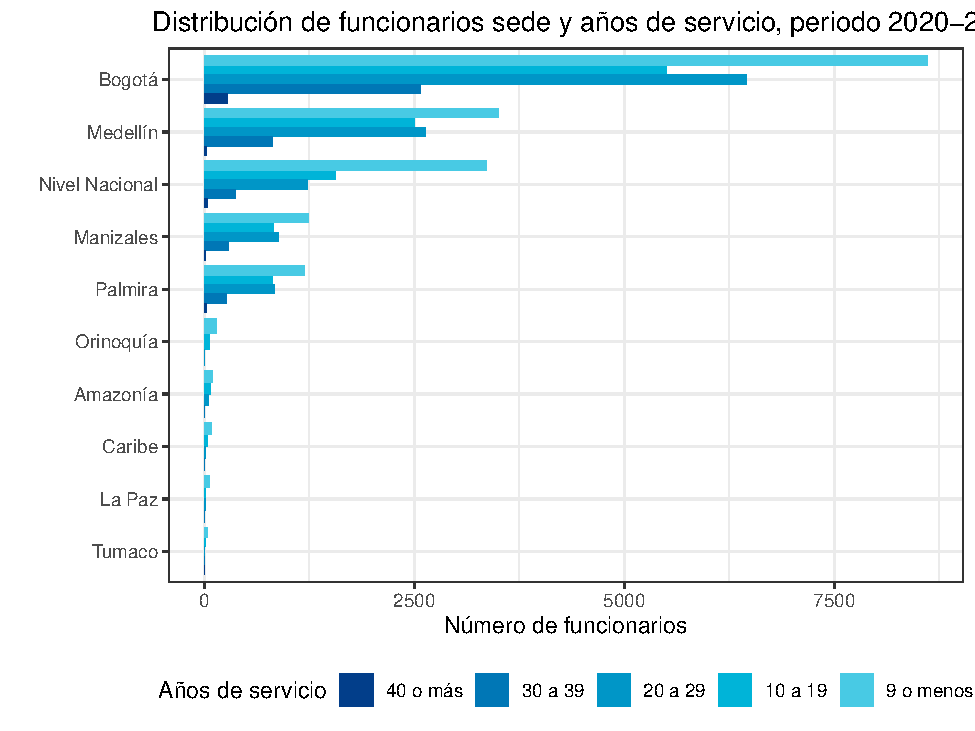
\includegraphics[width=0.8\linewidth]{Lineamientos-Visualizar_files/figure-latex/barrasagrupadassedeservicio-fig-1} 

}

\caption{Cantidad de funcionarios por sede y años de servicio}\label{fig:barrasagrupadassedeservicio-fig}
\end{figure}

Como ya vimos los gráficos de barras agrupadas consisten en dibujar una barra al lado de la otra, pero hay ocasiones en las cuales se prefiere apiliar las barras, es decir, ubicar una encima de la otra, esto generalmente se realiza cuando la cantidad representada por las barras dispuestas en esta posición es significativa, también es necesario tener cuidado con este tipo de gráficos ya que utilizar muchas categorías para apilar las barras resultara en una visualización saturada y poco informativa. Un uso común de este tipo de gráficos es cuando las barras individuales representan recuentos, por ejemplo, el conjunto de datos llamado Administrativos posee el recuento de funcionarios por sexo, para este caso si apilamos una barra que representa el recuento de mujeres encima de una barra que representa el recuento de hombres, entonces la altura de la barra combinada mostrara el total de funcionarios independiente del género. La figura \ref{fig:barrasaplidasserviciosexo-fig} presenta el uso de barras apiladas como alternativa del uso de barras agrupadas ilustrado en la figura \ref{fig:barrasagrupadasservicioedad-fig}.

\begin{figure}

{\centering 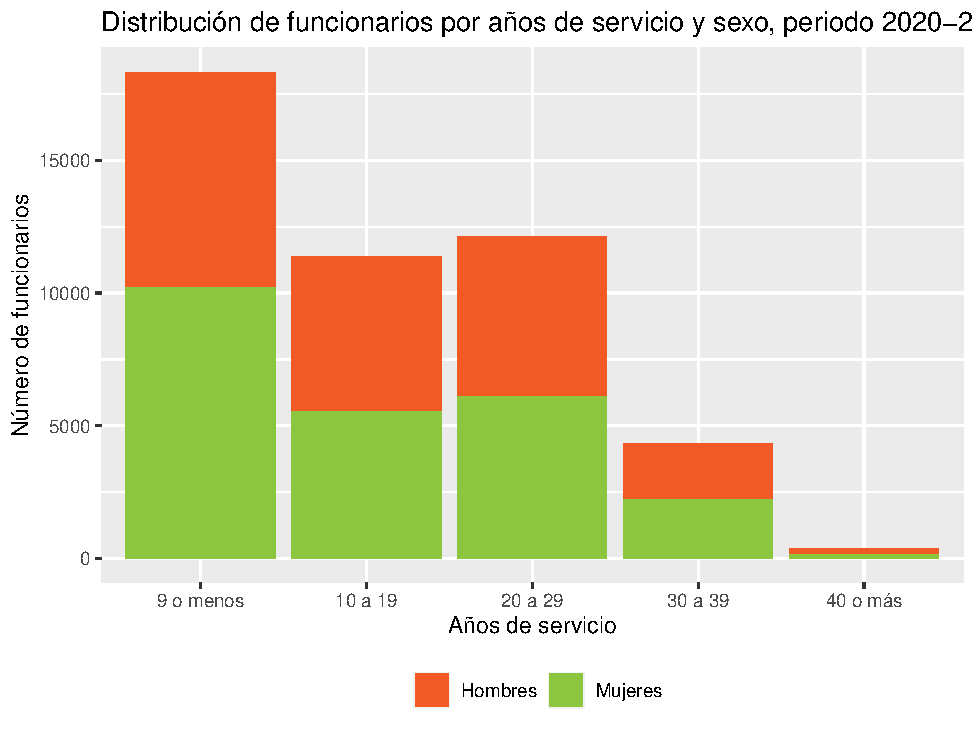
\includegraphics[width=0.8\linewidth]{Lineamientos-Visualizar_files/figure-latex/barrasaplidasserviciosexo-fig-1} 

}

\caption{Barras apiladas como una alternativa a las barras agrupadas}\label{fig:barrasaplidasserviciosexo-fig}
\end{figure}

\hypertarget{gruxe1ficos-de-puntos-y-mapas-de-calor}{%
\subsection{Gráficos de puntos y mapas de calor}\label{gruxe1ficos-de-puntos-y-mapas-de-calor}}

Una de las mayores limitaciones al usar los gráficos de barras ya sean simples o alguna de sus variaciones es que los ejes deben iniciar en cero para lograr que la altura de la barra sea proporcional a la cantidad que representa, existen muchas ocasiones en las cuales es poco práctico iniciar siempre los ejes en cero y una alternativa es usar puntos ubicados en lugares apropiados a lo largo del eje X o Y.

Suponga que se quiere visualizar la edad promedio de los estudiantes graduados por nivel de formación, observe que en este caso no tiene mucho sentido iniciar el eje Y en cero ya que la edad promedio estará por encima de los 20 años aproximadamente y las discrepancias entre los promedios de edades no son muy grandes, por esta razón es conveniente restringir el dominio de eje x al intervalo de 20 a 40 años, para que las diferencias sean notorias y la información sea interpretada con mayor facilidad, como se ilustra en la figura \ref{fig:diagramapuntos-fig}.

\begin{figure}

{\centering 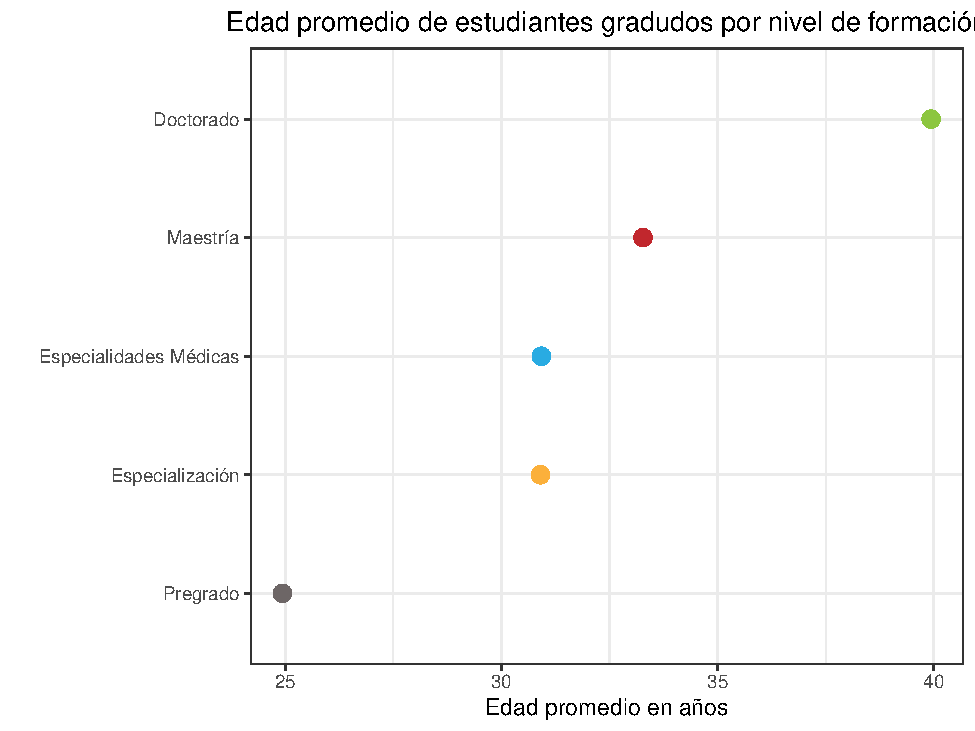
\includegraphics[width=0.8\linewidth]{Lineamientos-Visualizar_files/figure-latex/diagramapuntos-fig-1} 

}

\caption{Diagrama de puntos como alternativa a los gráficos de barras}\label{fig:diagramapuntos-fig}
\end{figure}

La figura \ref{fig:barrasedadpromedio-fig} muestra la edad promedio de los estudiantes graduados por nivel de formación usando un gráfico de barras, esta figura fue etiquetada como incorrecta ya que al usar barras el eje debe iniciar en cero y las discrepancias existentes entre las edades promedios de los niveles especialidades médicas y especialización no se logra apreciar con claridad.

\begin{figure}

{\centering 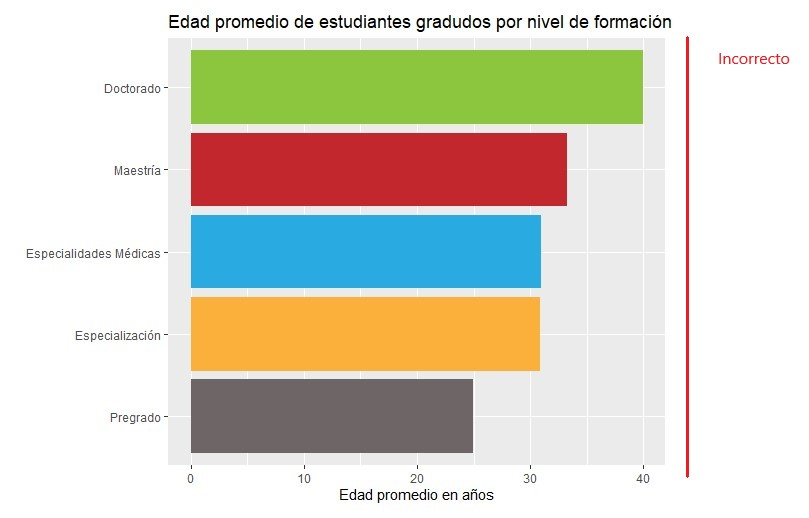
\includegraphics[width=1\linewidth]{Imágenes/edadpromediograduados} 

}

\caption{Edad promedio de estudiantes graduados}\label{fig:barrasedadpromedio-fig}
\end{figure}

Para este tipo de visualización también aplica reordenar las categorías por la variable numérica si las categorías no tienen un orden natural, este grafico es recomendable cuando no se tiene un orden natural en los datos ya que pueden ser reordenados logrando una visualización atractiva y entendible.

Las visualizaciones presentadas hasta el momento representan variables numéricas usando categorías a través de las posiciones en uno de los ejes, ya sea con un punto final en el valor que representa o el tamaño de la barra. Sin embargo, estos gráficos no son adecuados cuando el conjunto de datos muy grandes, ya que la cantidad de barras será excesiva y proporcionará una figura saturada. Ya se había observado en la figura \ref{fig:barrasagrupadasserviciosede-fig} que grupos de 8 barras resultan en una visualización compleja y no tan fácil de interpretar, imagine que en lugar de 8 barras por grupo se tuvieran 20 o más, resultaría aun más complejo y probablemente muy confusa.

Una alternativa a las barras y puntos son los mapas de calor, los cuales están formados por dos variables categóricas, una en cada eje, y los valores son representados a través de una escala de color secuencial. La figura \ref{fig:mapadecalor-fig} utiliza este enfoque para mostrar el número de accidentes ocurridos por día y mes en los años 2014 a 2016, es una figura útil para detectar tendencias más amplias que para visualizar exactamente cada uno de los valores que representa, se identifica con claridad que los primeros 15 días del mes de enero se presenta menor accidentalidad comparado con los días restantes de este mismo mes.

\begin{figure}

{\centering 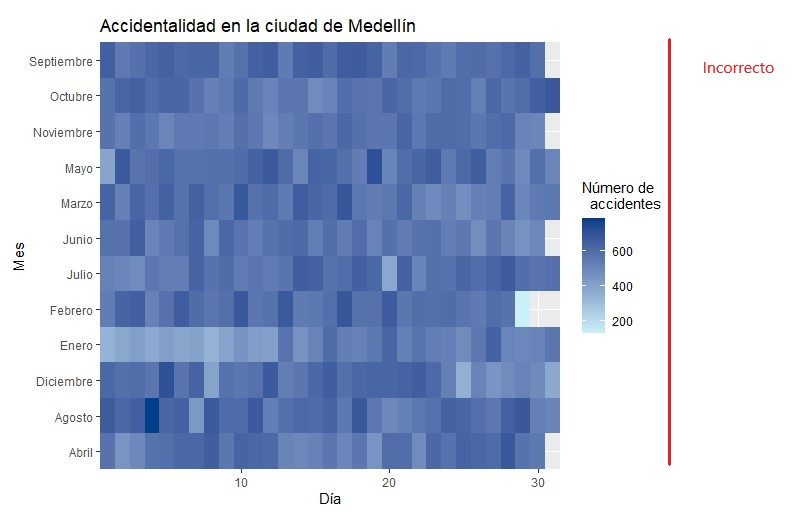
\includegraphics[width=1\linewidth]{Imágenes/mapadecalor} 

}

\caption{Mapa de calor para representar la accidentalidad en la ciudad de Medelllín}\label{fig:mapadecalor-fig}
\end{figure}

La figura \ref{fig:mapadecalor-fig} es informativa pero incorrecta ya que no se respeta el orden natural que poseen los datos, la figura correcta para visualizar los datos usando un mapa de calor se presenta a continuación.

\begin{figure}

{\centering 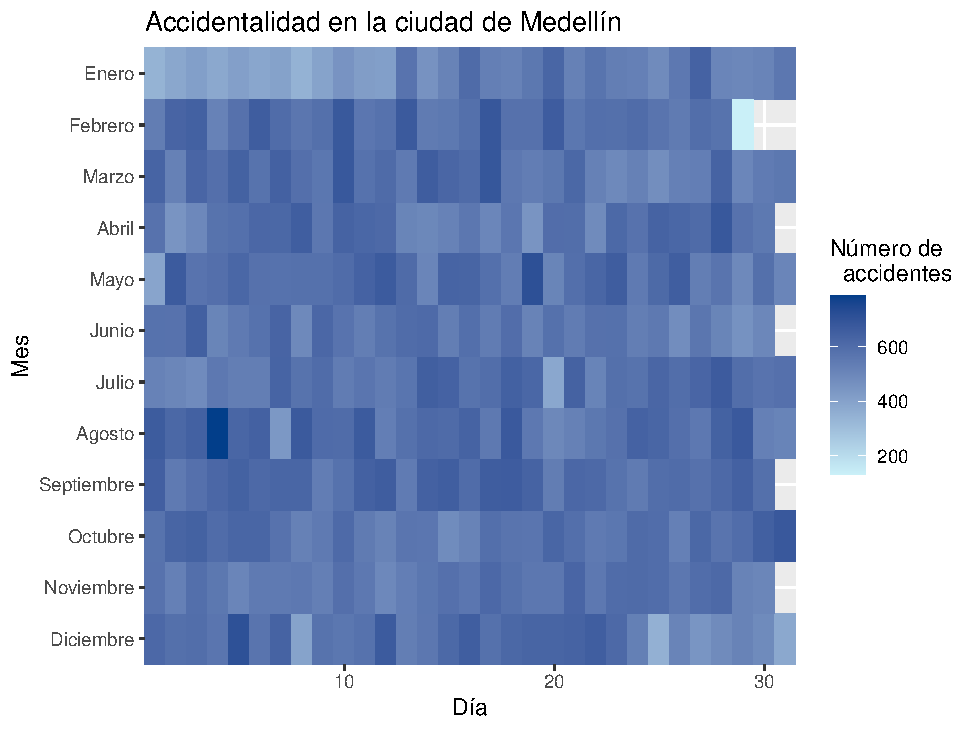
\includegraphics[width=0.8\linewidth]{Lineamientos-Visualizar_files/figure-latex/mapadecalorcorrecto-fig-1} 

}

\caption{Mapa de calor para representar la accidentalidad en la ciudad de Medelllín}\label{fig:mapadecalorcorrecto-fig}
\end{figure}

Como ya se ha mencionado en múltiples ocasiones se debe prestar mucha atención al orden de las variables categóricas, en este caso dichas variables presentan un orden natural ya que son meses y días, en el caso de no presentarse un orden natural podría reordenarse las categorías usando la variable numérica para lograr una visualización mas clara, atractiva y estéticamente llamativa.

\hypertarget{visualizaciuxf3n-de-proporciones}{%
\section{Visualización de proporciones}\label{visualizaciuxf3n-de-proporciones}}

Cuando se están analizando datos se presentan ocasiones en las cuales se quiere representar como algún grupo se divide en partes individuales que representan un porcentaje o proporción de un todo, entre los ejemplos más comunes se incluyen las proporciones de hombres y mujeres dentro de un grupo de personas, el porcentaje de estudiantes graduados por modalidad de formación, el porcentaje de estudiantes admitidos por facultad en cada una de las sedes de la Universidad Nacional de Colombia, entre muchos otros ejemplos.

La visualización más utilizada en este caso es el gráfico circular, gráfico odiado y amado por muchos, el éxito de este gráfico depende principalmente de la correcta elección de grupos y colores. Cuando el todo se divide en muchas partes diferentes o cuando queremos ver los cambios en las proporciones a través de una ventana de tiempo mostrar las proporciones se convierte en un verdadero reto y no hay una visualización única que funcione en todos los casos.

Generalmente para mostrar proporciones se usan gráficos circulares, barras apiladas y barras una al lado de la otra, dependiendo del propósito de la visualización se elige cada una de las opciones mencionadas.

\hypertarget{gruxe1ficos-circulares}{%
\subsection{Gráficos circulares}\label{gruxe1ficos-circulares}}

Un gráfico circular está compuesto de una variable discreta que determina la cantidad de divisiones del circulo y adicionalmente una variable numérica con la cual se generan los fragmentos y se debe lograr que cada uno sea proporcional a la fracción del total que representa.

Dentro de los datos almacenados para los estudiantes admitidos a la Universidad Nacional se encuentra el estrato socioeconómico el cual está dividido o categorizado en tres grupos, en este caso es posible usar un gráfico circular como se ilustra en la figura \ref{fig:circularcorrecto-fig}, se observa que del total de estudiantes admitidos el \(50.91\%\) pertenece al grupo de estrado 2 o menos, el \(32.88\%\) al estrato 3 y el restante a la categoría de estrato 4 o más.

\begin{figure}

{\centering 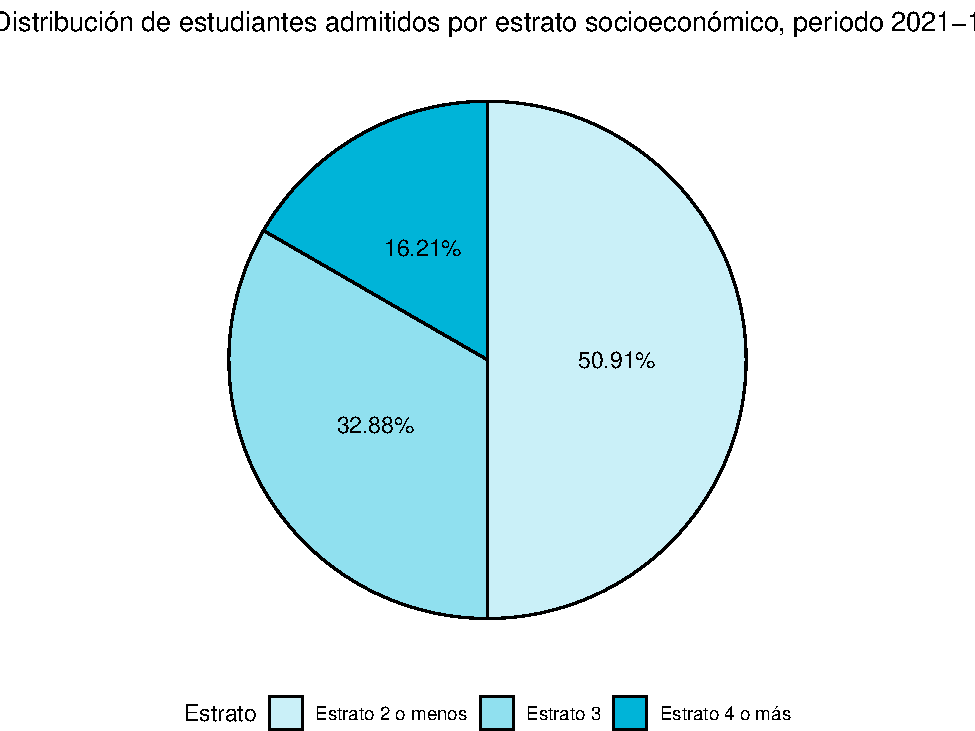
\includegraphics[width=0.8\linewidth]{Lineamientos-Visualizar_files/figure-latex/circularcorrecto-fig-1} 

}

\caption{Gráfico circular para representar 3 categorías}\label{fig:circularcorrecto-fig}
\end{figure}

La figura anterior se considera como un uso correcto de los gráficos circulares ya que estos son recomendados para visualizar los datos como proporciones de un todo y enfatizar visualmente en fracciones simples como la mitad, un tercio o un cuarto, es decir, funciona correctamente cuando la cantidad de divisiones no es mayor a cuatro o cinco y es posible utilizarlo en conjuntos de datos pequeños.

Cuando se tienen variables con muchas categorías no se recomienda utilizar los gráficos circulares ya que no se logra enfatizar en las proporciones y las etiquetas de cada categoría no se observan con claridad, la figura \ref{fig:circularincorrecto-fig} se considera un uso incorrecto de los gráficos circulares ya que la variable discreta utilizada tiene nueve categorías, para esta ocasión se prefiere un gráfico de barras, aunque se pierdan algunas características como la relación con el total.

\begin{figure}

{\centering 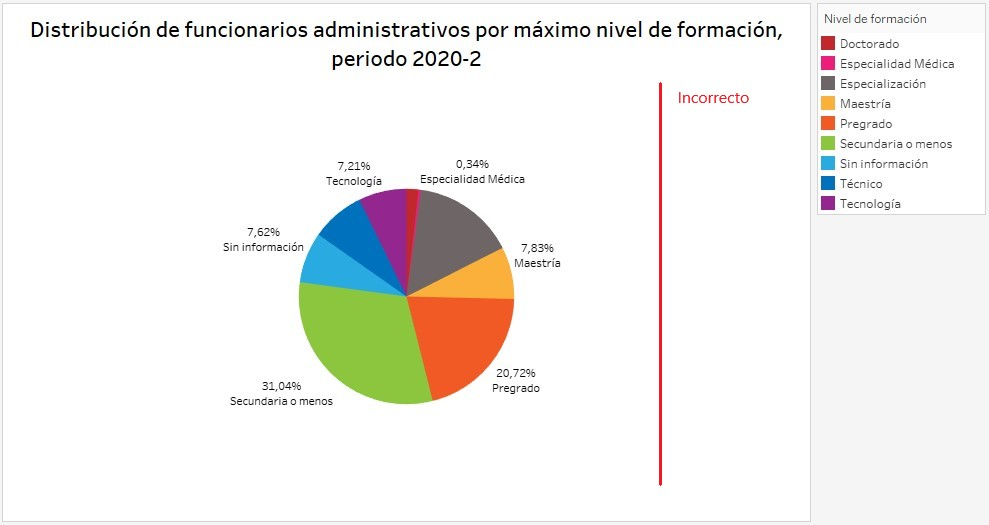
\includegraphics[width=1\linewidth]{Imágenes/circularincorrecto} 

}

\caption{Uso incorrecto de los gráficos circulares}\label{fig:circularincorrecto-fig}
\end{figure}

\hypertarget{errores-en-la-trama}{%
\chapter{Errores en la trama}\label{errores-en-la-trama}}

El principal y más grande error dentro de la visualización de datos es no respetar la integridad gráfica, por integridad gráfica nos referimos a los factores de engaño o adornos que se añaden, pensando que harán las figuras más atractivas y llamativas, pero en realidad saturan y opacan la verdadera intención de los gráficos que es informar. Un ejemplo claro de esto son las figuras 3D, las rejillas y los rellenos con patrones.

El factor de engaño corresponde a las distorsiones generadas por la mala elección de los elementos gráficos, también se incluyen elementos gráficos que no corresponden a variaciones de datos o que hacen más compleja la interpretación de estos.

Un diseño muy popular que introduce una alta distorsión en los datos son los gráficos en 3D, muchos softwares de visualización permiten arreglar los gráficos convirtiéndolos en objetos tridimensionales que generalmente son rotados hasta conseguir una proyección bidimensional, comúnmente este efecto es aplicado a gráficos de torta, barras y dispersión. El principal problema con los diseños 3D es que la proyección a dos dimensiones para poder visualizarlos en un monitor distorsiona los datos, para ilustrar esto observe la figura \ref{fig:circular3d-fig} que muestra la distribución de aspirantes a pregrado del programa PAES para el periodo 2021-1, note que la rebana correspondiente a la población afrocolombiana se ve más grande que la rebanada de comunidades indígenas, aunque claramente este no es el caso, ya que de los aspirantes a pregrado el \(26\%\) pertenece a comunidades indígenas y el \(17\%\) a la población afroamericana. Este es un claro ejemplo de los factores de engaño que se pueden introducir al gráfico a través de elementos estéticos como el diseño tridimensional.

\begin{figure}

{\centering 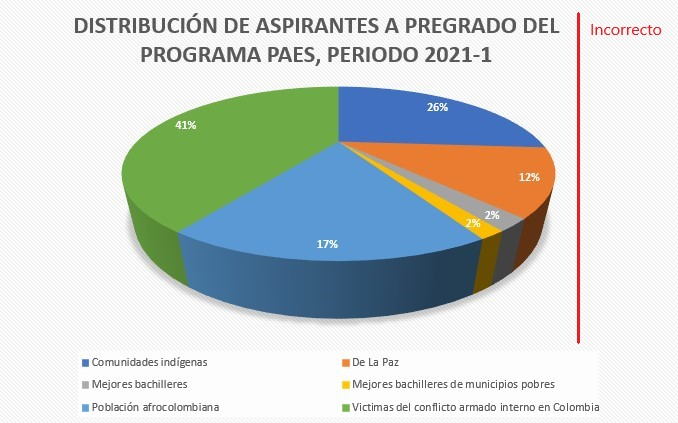
\includegraphics[width=1\linewidth]{Imágenes/circular3d} 

}

\caption{Uso incorrecto de las figuras en 3D}\label{fig:circular3d-fig}
\end{figure}

Para eliminar el factor de engaño es necesario eliminar de la visualización el efecto 3D, para lograr que cada rebanada sea proporcional a cantidad que representa, como se muestra en la figura \ref{fig:circularpaes-fig}, a pesar de que esta visualización es mucho más clara que la anterior no es del todo correcta, ya que la variable discreta presenta seis categorías y este tipo de gráficos es recomendable cuando no se superan las cuatro categorías.

\begin{figure}

{\centering 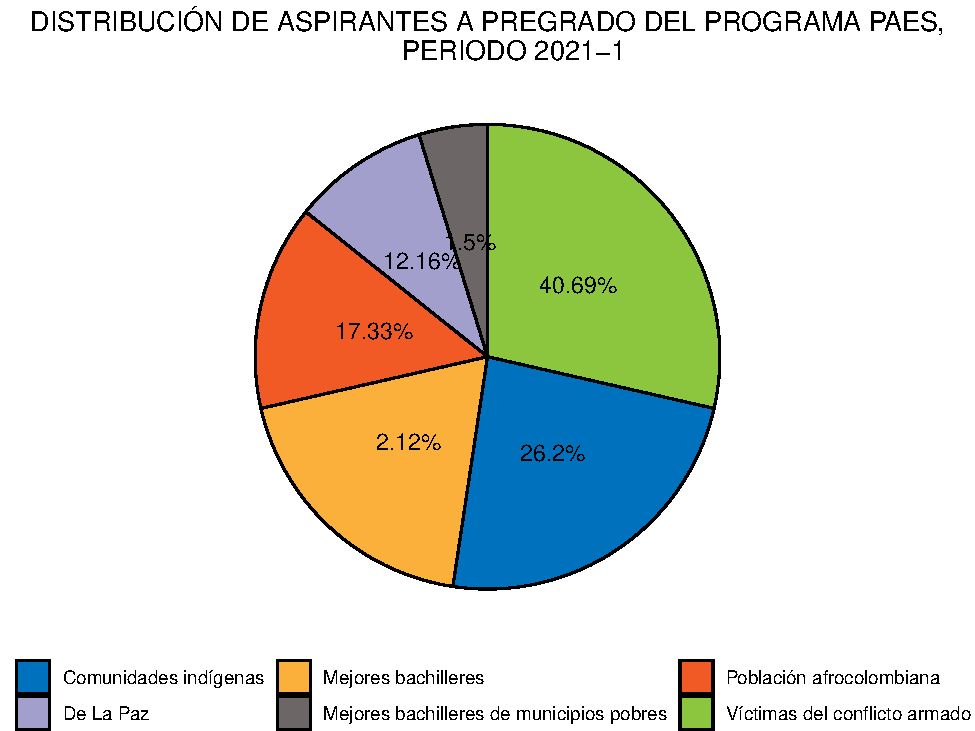
\includegraphics[width=0.8\linewidth]{Lineamientos-Visualizar_files/figure-latex/circularpaes-fig-1} 

}

\caption{Eliminar efecto 3D}\label{fig:circularpaes-fig}
\end{figure}

Cuando se presentan más de cuatro categorías es recomendable utilizar un gráfico de barras y ordenar las clases de manera decreciente para lograr una mejor comprensión por parte del usuario.

En muchas ocasiones cuando se realizan gráficos de dispersión se opta por añadir rejillas con la intención de que el usuario identifique con facilidad las coordenadas X y Y de las observaciones, pero es común usar colores muy fuertes para estas rejillas opacando por completo las observaciones, como se ilustra en la figura \ref{fig:usoderejillas-fig}.

\begin{figure}

{\centering 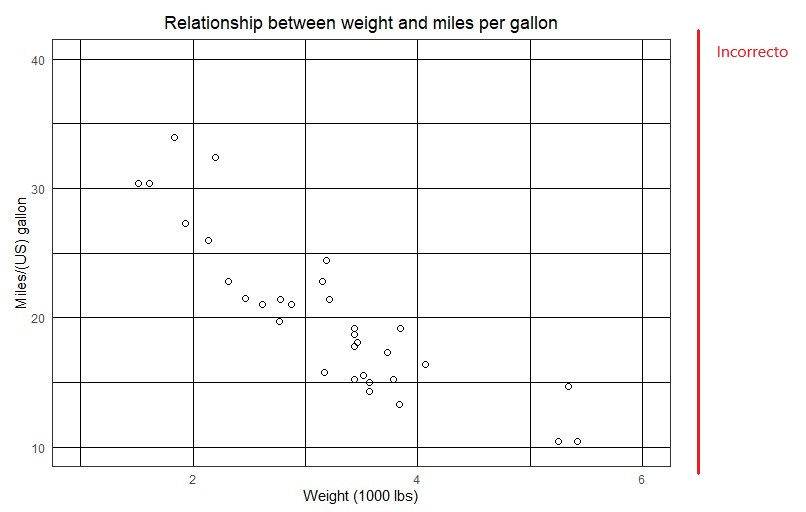
\includegraphics[width=1\linewidth]{Imágenes/rejillas} 

}

\caption{Uso incorrecto de rejillas}\label{fig:usoderejillas-fig}
\end{figure}

La figura \ref{fig:usoderejillas-fig} representa la relación existente entre el peso en miles de libras y la distancia recorrida en millas por galón para 32 autos, esta figura es etiquetada como incorrecta ya que la rejilla se sobrepone a las observaciones creando una visualización saturada, poco comprensible y degrada la percepción de patrones en los datos. Lo recomendado en estas ocasiones es utilizar puntos rellenos y colores suaves para la rejilla por ejemplo tonalidades grises como se presenta en la figura \ref{fig:rejillagris-fig}.

\begin{figure}

{\centering 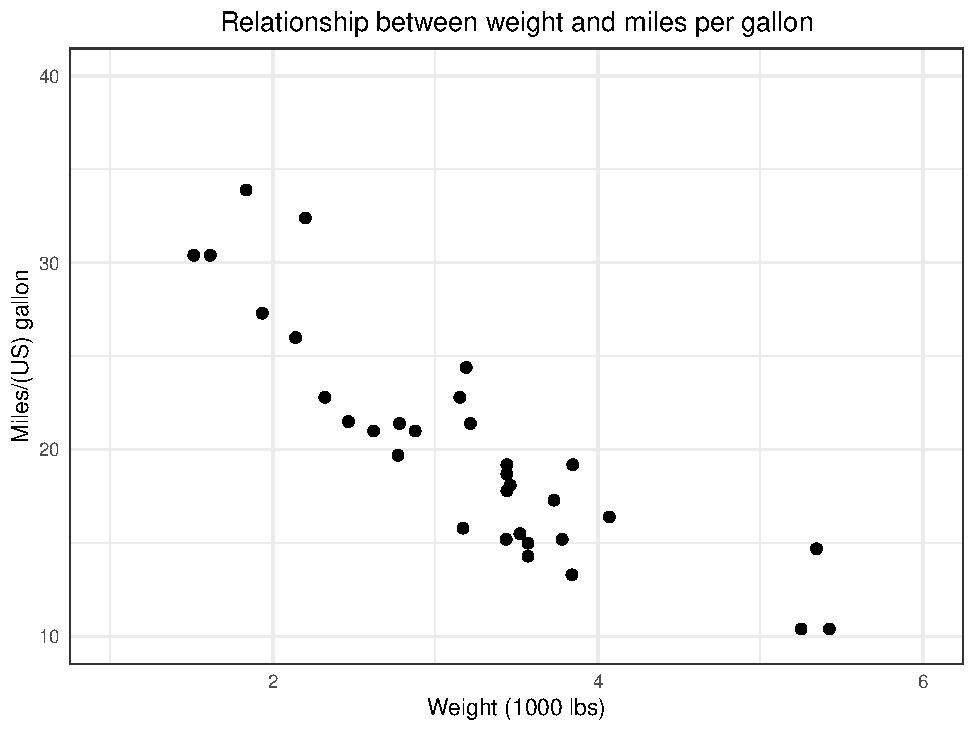
\includegraphics[width=0.8\linewidth]{Lineamientos-Visualizar_files/figure-latex/rejillagris-fig-1} 

}

\caption{Uso de rejillas en tonalidades suaves}\label{fig:rejillagris-fig}
\end{figure}

Otro adorno comúnmente utilizado que es desagradable y quita la atención de los datos es usar patrones para rellenar las figuras, por ejemplo, utilizar líneas, puntos, estrellas u otras figuras para rellenar las barras, la figura \ref{fig:barrasconpatrones-fig} muestra la distribución de los graduados por grupo de edad para el periodo 2020-2, se etiqueto como incorrecta ya que añadir patrones para rellenar las barras se considera poco atractivo y distrae la atención del usuario.

\begin{figure}

{\centering 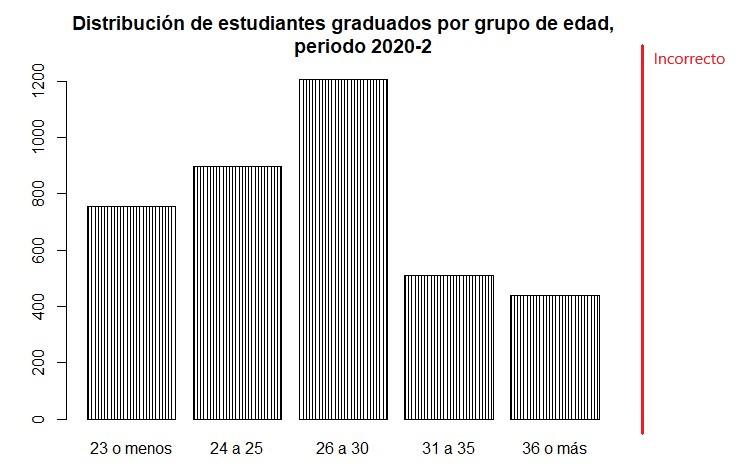
\includegraphics[width=1\linewidth]{Imágenes/barrasconpatrones} 

}

\caption{Uso incorrecto de los patrones para rellenar}\label{fig:barrasconpatrones-fig}
\end{figure}

Cuando se quiere añadir algún tipo de relleno a las barras se recomienda hacerlo con colores, usando escalas de colores cualitativas si la intención es distinguir datos o una escala secuencial si se trata de representar cantidades, la forma correcta o recomendada para realizar esta gráfica se muestra en la figura \ref{fig:graduadosporgrupoedadcorrecto-fig}.

\begin{figure}

{\centering 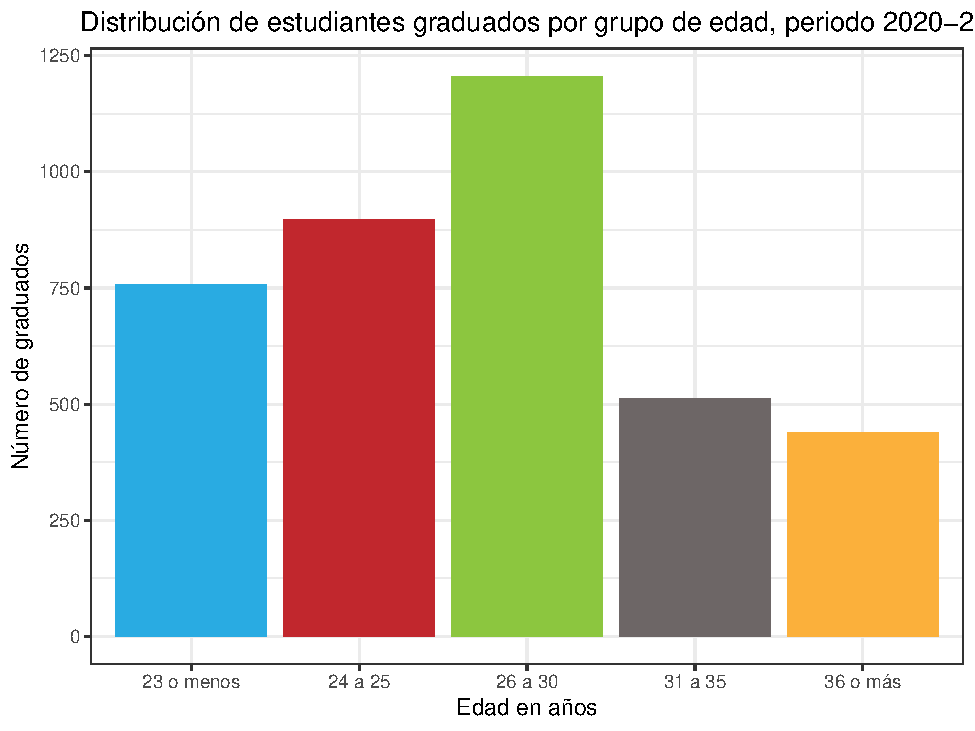
\includegraphics[width=0.8\linewidth]{Lineamientos-Visualizar_files/figure-latex/graduadosporgrupoedadcorrecto-fig-1} 

}

\caption{Uso de los rellenos de color}\label{fig:graduadosporgrupoedadcorrecto-fig}
\end{figure}

\hypertarget{final-words}{%
\chapter{Final Words}\label{final-words}}

We have finished a nice book.

  \bibliography{book.bib,packages.bib}

\end{document}
